\documentclass[final,hidelinks,onefignum,onetabnum]{siamart250211}
%\documentclass[review,hidelinks,onefignum,onetabnum]{siamart250211}

\usepackage{amsfonts,amssymb}
\usepackage{graphicx}
\ifpdf
  \DeclareGraphicsExtensions{.eps,.pdf,.png,.jpg}
\else
  \DeclareGraphicsExtensions{.eps}
\fi
\usepackage{bm}
\usepackage{tikz}
\usetikzlibrary{math,positioning}

% Add a serial/Oxford comma by default.
\newcommand{\creflastconjunction}{, and~}

% Used for creating new theorem and remark environments
\newsiamremark{remark}{Remark}
\newsiamthm{stdass}{Standard Assumptions}
\newsiamthm{conjecture}{Conjecture}

\DeclareMathOperator{\diag}{diag}

\newcommand{\eps}{\epsilon}
\newcommand{\RR}{\mathbb{R}}

\newcommand{\grad}{\nabla}
\newcommand{\Div}{\nabla\cdot}

\newcommand{\bbf}{\mathbf{f}}
\newcommand{\bg}{\mathbf{g}}
\newcommand{\bn}{\mathbf{n}}
\newcommand{\bu}{\mathbf{u}}
\newcommand{\bv}{\mathbf{v}}
\newcommand{\bw}{\mathbf{w}}
\newcommand{\bx}{\mathbf{x}}
\newcommand{\bz}{\mathbf{z}}

\newcommand{\bU}{\mathbf{U}}
\newcommand{\bX}{\mathbf{X}}

\newcommand{\bzero}{\bm{0}}

\newcommand{\btau}{\bm{\tau}}

\newcommand{\cB}{\mathcal{B}}
\newcommand{\cH}{\mathcal{H}}
\newcommand{\cK}{\mathcal{K}}
\newcommand{\cQ}{\mathcal{Q}}
\newcommand{\cT}{\mathcal{T}}
\newcommand{\cV}{\mathcal{V}}
\newcommand{\cX}{\mathcal{X}}

\newcommand{\hcK}{\widehat{\cK}}

\newcommand{\nn}{{\text{\textnormal{n}}}}
\newcommand{\pp}{{\text{\textnormal{p}}}}
\newcommand{\qq}{{\text{\textnormal{q}}}}
\newcommand{\rr}{{\text{\textnormal{r}}}}

\newcommand{\ip}[2]{\left<#1,#2\right>}

\newcommand{\XX}{\ding{55}}

\newcommand{\dx}{\, \mathrm{d}x}

\newcommand{\rhoi}{\rho_{\text{i}}}

\newcommand{\nsubset}{\not\subset}
\DeclareMathOperator*{\argmin}{arg\,min}
\DeclareMathOperator*{\Hull}{Hull}

\newcommand{\Vdiv}{\cV_{\text{\textnormal{div}}}}

\newcommand{\CA}{C_\text{\textnormal{A}}}


% Optional PDF information
\ifpdf
\hypersetup{
  pdftitle={Surface elevation errors in finite element Stokes models for glacier evolution},
  pdfauthor={E. Bueler}
}
\fi

% Sets running headers as well as PDF title and authors
\headers{Surface elevation errors in glacier models}{E. Bueler}

% Title.
\title{Surface elevation errors in finite element Stokes models for glacier evolution\thanks{Submitted to the editors DATE (draft \today).}}

% Authors: full names plus addresses.
\author{Ed Bueler\thanks{Dept.~Mathematics \& Statistics, University of Alaska Fairbanks, USA (\email{elbueler@alaska.edu}, \href{https://bueler.github.io/}{\texttt{bueler.github.io}}).}}

% FundRef data to be entered by SIAM
%<funding-group specific-use="FundRef">
%<award-group>
%<funding-source>
%<named-content content-type="funder-name">
%</named-content>
%<named-content content-type="funder-identifier">
%</named-content>
%</funding-source>
%<award-id> </award-id>
%</award-group>
%</funding-group>


\begin{document}

\maketitle

\begin{abstract}
The primary data which determine the evolution of glaciation are the bedrock elevation and the surface mass balance.  From this data, which we assume is defined over a fixed land region, the glacier's geometry solves a free boundary problem which balances the time derivative of the surface elevation, the surface velocity from the Stokes flow of the ice, and the surface balance rate.  This problem can be posed in weak form as a variational inequality over a cone of admissible surface elevation functions, those which are above the bedrock topography.  After some preparatory theory for the Stokes problem, we conjecture that the corresponding continuous-space, implicit time-step variational inequality problem is well-posed if the surface kinematical equation is appropriately regularized.  This conjecture is supported by physical arguments and numerical evidence.  We then prove a general theorem which bounds the numerical error made by finite element approximations of nonlinear-operator variational inequalities in Banach spaces.  This bound is a sum of error terms of different types, special to variational inequalities.  When it is applied to our implicit time-step glacier problem there are three terms in the bound: an error from discretizing the bed elevation, an error from numerically solving for the Stokes velocity, and finally an expected error which is quasi-optimal in the finite element space representation of the surface elevation.  The design of glacier models is then reconsidered, based on this \emph{a priori} error analysis.
\end{abstract}

\begin{keywords}
error bounds, finite element methods, glaciers, ice flow, variational inequalities
\end{keywords}

\begin{MSCcodes}
76D27, 76D07, 49J40, 65N30, 65N15
\end{MSCcodes}


\section{Introduction} \label{sec:intro}

Glacier and ice sheet simulations model the flowing ice as a free-surface layer of very-viscous, incompressible, and non-Newtonian fluid \cite{GreveBlatter2009,SchoofHewitt2013}.  The two essential input data into such simulations are the bedrock elevation, which is assumed here to be independent of time, and the time- and space-dependent surface mass balance rate (SMB), the climate.  By definition, the SMB is the balance between accumulating snow and the loss of melt water, through runoff, at the upper surface of the glacier \cite{Cogleyetal2011}.  Here we will only consider simulations of land-based glaciers and ice sheets (continent-scale glaciers), without floating portions.  Note that elevations are measured in meters, and SMB is in (ice-equivalent) meters per second.

Thus a glacier simulation takes, as inputs, a bedrock topography, a climate, and an initial glacier geometry.  The simulation produces the glacier's evolving geometry and flow velocity.  Comprehensive models  \cite{SchoofHewitt2013,Winkelmannetal2011} generally have additional physics.  For example, they might track the enthalpy/temperature \cite{Aschwandenetal2012} of the ice, or liquid water along glacier surfaces.  However, for relative simplicity in the current work, we only consider conservation of mass and momentum, but not energy, and liquid water plays no role.  Furthermore we will assume zero velocity at the base of the ice, a non-sliding and non-penetrating condition.  On the other hand, we will not make any of the shallowness assumptions which are common in present-day comprehensive models, and we will address the mathematical evolution model rigorously.

One may parameterize the glacier's geometry using either the (upper) surface elevation or the ice thickness.  At any time and map-plane location where a glacier exists the surface elevation of the ice exceeds the elevation of the bedrock, equivalently the ice thickness is positive.  The computed flow velocity is only defined at those locations and times where ice is present, on an evolving 3D domain between the bedrock and surface elevations.  In other words, admissibility of the surface elevation is required to make the velocity and pressure Stokes problem meaningful.

The kinematical notation which we need is sketched in Figure \ref{fig:stokesdomain}.  Let $\Omega \subset \RR^2$ be a fixed portion of land, an open and connected set, with map-plane coordinates $x=(x_1,x_2)\in\Omega$.  We assume that we are given, as data, a continuous bedrock elevation function $b(x)$ on $\Omega$, and a continuous SMB function $a(t,x)$ on $[0,T]\times \Omega$, for some $T>0$.  Where $a>0$ (accumulation; downward arrows in Figure \ref{fig:stokesdomain}), a glacier will exist.  However, where $a<0$ (ablation; upward arrows) then either ice exists with an ablating surface, generally supported by flow from accumulation areas, or no glacier exists.  Determining which situation applies at some coordinates $t,x$, and determining the surface elevation there, requires solving a free-boundary problem.

\begin{figure}[ht]
\centering
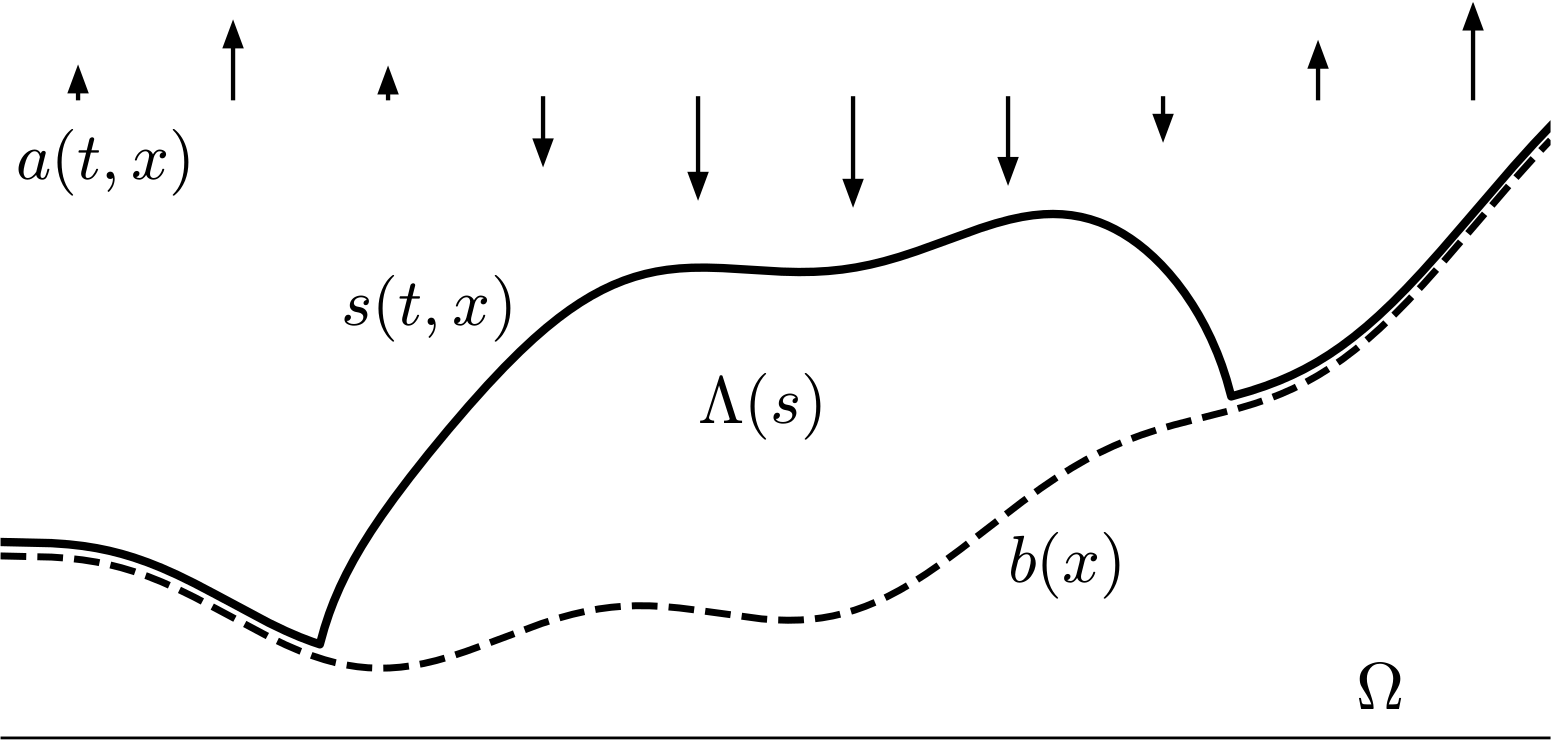
\includegraphics[width=0.6\textwidth]{genfigs/stokesdomain.pdf}
\caption{Glacier notation: $x\in\Omega\subset\RR^2$ and $\Lambda(t)\subset\RR^3$.}
\label{fig:stokesdomain}
\end{figure}

Let $s(t,x)$ be the (solution) ice surface elevation.  This is defined for all $x\in\Omega$, but subject to the constraint that the surface $z=s$ must be at or above the bedrock ($s \ge b$).  In regions with no ice, $s=b$ holds.  The solution ice velocity $\bu(t,x,z)$ and pressure $p(t,x,z)$ are then defined only on the open 3D domain
\begin{equation}
\Lambda(t) = \left\{(x,z)\,:\,b(x) < z < s(t,x)\right\} \subset \Omega \times \RR. \label{eq:icydomain}
\end{equation}
This aspect of glacier modeling deserves emphasis:  The time-dependent 3D domain $\Lambda(t)$, on which the velocity and pressure are meaningful, is determined by the evolving surface elevation $s$, which is itself part of the coupled model solution.

The surface trace of the ice velocity will be of importance, with a precise Sobolev space for the velocity given in Section \ref{sec:stokes}.  We extend it by zero so that it is defined for all $t,x \in [0,T]\times\Omega$; compare flux extension by zero in \cite{SchoofHewitt2013}:
\begin{equation}
\bu|_s(t,x) = \begin{cases} \bu(t,x,s(t,x)), & s(t,x)>b(t,x) \\
                            \bzero, & \text{otherwise} .\end{cases} \label{eq:defineus}
\end{equation}
Also let $\bn_s = \left<-\partial s/\partial x_1,-\partial s/\partial x_2,1\right>$ denote an upward surface normal vector, assumed well-defined for this Introduction.

The glacier geometry evolution model now says that an infinite-dimensional nonlinear complementarity problem (NCP) \cite{FacchineiPang2003}, an obstacle problem, applies in $[0,T]\times \Omega$:
\begin{subequations}
\label{eq:ncp}
\begin{align}
s - b &\ge 0 \label{eq:ncp:constraint} \\
\frac{\partial s}{\partial t} - \bu|_s \cdot \bn_s - a &\ge 0 \label{eq:ncp:residualpos} \\
(s - b) \left(\frac{\partial s}{\partial t} - \bu|_s \cdot \bn_s - a\right) &= 0
\end{align}
\end{subequations}

System \eqref{eq:ncp} implies that either a location is ice free ($s=b$), where the climate is locally ablating ($a\le 0$), or that the surface kinematical equation (SKE) holds:
\begin{equation}
\frac{\partial s}{\partial t} - \bu|_s \cdot \bn_s - a = 0.  \label{eq:ske}
\end{equation}
This equation says that the (non-material) ice surface moves vertically according to the sum of an ice velocity component at the surface and the SMB.  This statement of mass conservation \cite{Aschwandenetal2012}, also called the free-surface equation \cite{LofgrenAhlkronaHelanow2022}, is a standard description of glacier geometry evolution in numerical models \cite{GreveBlatter2009,SchoofHewitt2013}.  Glaciologists would agree with the conditions of NCP \eqref{eq:ncp}, though it is not yet common to state it completely in this way.  While condition \eqref{eq:ncp:constraint} is sometimes stated in glacier literature \cite{Durandetal2009,Halfar1981,JouvetBueler2012,PiersantiTemam2023,WirbelJarosch2020}, the complementary fact \eqref{eq:ncp:residualpos}, that the residual is everywhere nonnegative, though observed in \cite{Calvoetal2003}, is rarely written \cite{SchoofHewitt2013}.

Because a simulated glacier needs to be able to advance into unglaciated locations, we assume that the SMB is defined everywhere in $\Omega$, regardless of whether a glacier is present or not.  In ice-free areas the input SMB should have the value which a glacier surface at elevation $b$ would experience.  It can be computed, from precipitation and an energy balance model \cite{GreveBlatter2009}, by balancing snow accumulation minus the ablation which would follow from using the available energy for melt if ice were present.

Let us address the non-shallow ice dynamics model used in this paper.  It is the non-sliding (e.g.~frozen base), isothermal, non-Newtonian, and incompressible Stokes system \cite{GreveBlatter2009,JouvetRappaz2011,SchoofHewitt2013}, applied over the domain $\Lambda(t)$ defined in \eqref{eq:icydomain}.  Let $\Gamma_s(t)$, $\Gamma_b(t)$ denote the upper and lower surfaces at $z=s$ and $z=b$, respectively.  The possibility of cliffs at the ice margin will be neglected, so $\partial \Lambda(t) = \overline{\Gamma_s(t)} \cup \overline{\Gamma_b(t)}$.  Let $D\bu=(\grad \bu + \grad \bu^{\top})/2$ denote the strain rate tensor, with Frobenius norm $|D\bu| = \left((D\bu)_{ij} (D\bu)_{ij}\right)^{1/2}$.  A shear-thinning constitutive relation, namely a regularized Glen's flow law \cite{GreveBlatter2009}, computes the effective dynamic ice viscosity by this formula:
\begin{equation}
\nu(D\bu) = \nu_\pp \left(|D\bu|^2 + \mu_0\right)^{(\pp-2)/2}. \label{eq:glen}
\end{equation}
The exponent $1 < \pp \le 2$, written $\pp=(1/\nn)+1$ in terms of Glen's exponent $\nn\ge 1$, is commonly taken to be $\pp=4/3$ \cite{GreveBlatter2009}.  The coefficient $\nu_\pp>0$ necessarily has $\pp$-dependent units, but $\nu(D\bu)$ has SI units $\text{kg}\,\text{m}^{-1}\,\text{s}^{-1}$.  The values of $\nn$ and $\nu_\pp$, assumed to be constant here, are constrained by laboratory experiments on ice \cite{GoldsbyKohlstedt2001,GreveBlatter2009}.  While $\pp=2$ yields a Newtonian fluid with constant viscosity, if $\pp < 2$ then the $\mu_0>0$ regularization implies that $\nu(D\bu)$ is bounded.

Now the velocity and pressure solve the following 3D fluid equations:%
\begin{subequations}
\label{eq:stokes}
\begin{align}
- \nabla \cdot \left(2 \nu(D\bu)\, D\bu\right) + \nabla p &= \rhoi \bg && \text{within $\Lambda(t)$} \\
\nabla \cdot \bu &= 0 && \qquad \text{''} \label{eq:stokes:incomp} \\
\left(2 \nu(D\bu) D\bu - pI\right) \bn_s &= \bzero && \text{on $\Gamma_s(t)$}\label{eq:stokes:stressfreesurface} \\
\bu  &= \bzero && \text{on $\Gamma_b(t)$} \label{eq:stokes:noslide}
\end{align}
\end{subequations}
The density of ice $\rhoi$ and the acceleration of gravity $\bg$ are here assumed constant.  Boundary condition \eqref{eq:stokes:stressfreesurface} says that the sub-aerial upper surface is stress free.\footnote{Though both apply on $\Gamma_s(t)$,  \eqref{eq:stokes:stressfreesurface} must not be confused with equation \eqref{eq:ske}.}  
The Stokes sub-problem \eqref{eq:glen}, \eqref{eq:stokes} is commonly discretized using finite elements (FEs) \cite{IsaacStadlerGhattas2015,Jouvetetal2008,Pattynetal2008}; we will return to the FE approximation in Chapter \ref{sec:application}.

In summary at this point, this work considers an evolving free-surface flow for a glacier, subject to a signed climate which can add or remove ice, simultaneously with a non-Newtonian Stokes problem which must be solved within the evolving 3D domain of ice.  This coupled initial-boundary value problem, in strong form as \eqref{eq:icydomain}--\eqref{eq:stokes}, requires data $b(x)$ and $a(t,x)$, plus an initial surface elevation $s(0,x)$.  The solution variables are $s(t,x)$, defined everywhere over $[0,T]\times \Omega$ and subject to $s \ge b$, and $\bu(t,x,z)$, and $p(t,x,z)$ defined only on $\Lambda(t)$ given by \eqref{eq:icydomain}.

A formulation using ice thickness to parameterize glacier geometry would have a different character from ours using surface elevation.  The latter is subject to a flow-caused smoothing effect, illustrated for a real ice sheet in Figure \ref{fig:giscross}.  For land-based glaciers $s(t,x)$ is spatially smoother than the thickness $H(t,x) = s(t,x)-b(x)$, which ``inherits'' the lower regularity of the often steep and eroded bedrock topography.

\begin{figure}
\begin{minipage}[t]{0.8\textwidth}
\vspace{0pt}
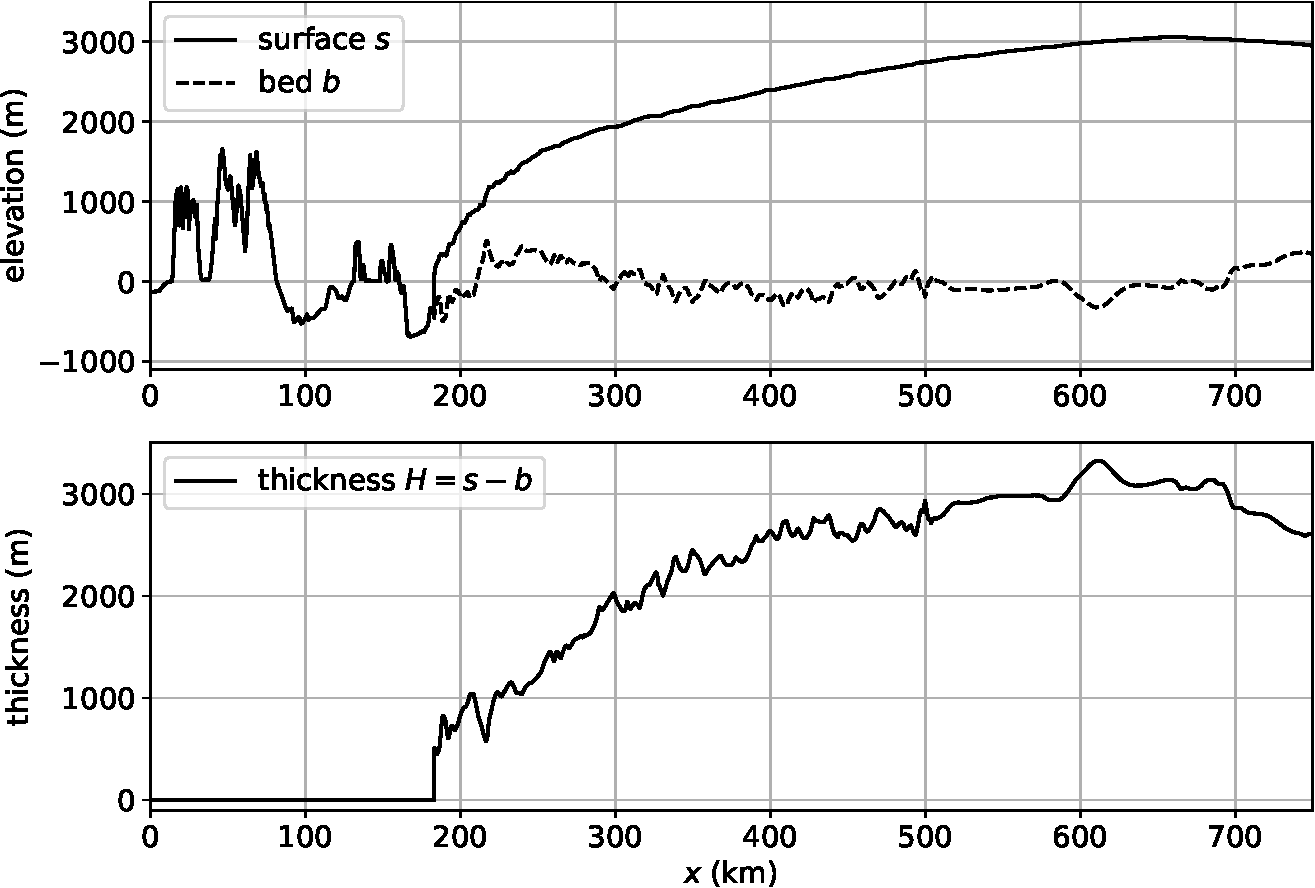
\includegraphics[width=\textwidth]{genfigs/giscross.pdf}
\end{minipage}
\,
\begin{minipage}[t]{0.15\textwidth}
\vspace{10pt}
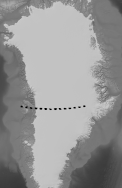
\includegraphics[width=\textwidth]{genfigs/gis/gris-profile-gray.png}
\end{minipage}
\caption{A cross-section of the Greenland ice sheet at $70^\circ$N latitude \cite{Morlighemetal2017}; see inset.  Top: While the ice surface $s$ is smoothed because of ice flow, the bedrock elevation $b$ is much rougher.  Bottom: The corresponding ice thickness $H = s-b$ ``inherits'' the low regularity of $b$.}
\label{fig:giscross}
\end{figure}

Observe that NCP \eqref{eq:ncp} is the only part of the model where a time derivative appears.  Indeed, because the flow is very-viscous \cite{Acheson1990}, the Stokes sub-model acts as an instantaneous ``algebraic'' constraint on the evolution.  Therefore this coupled and infinite-dimensional problem is simultaneously a differential algebraic equation (DAE) system \cite{AscherPetzold1998,LofgrenAhlkronaHelanow2022} and a free-boundary, obstacle-type NCP.

While this non-trivially coupled system is a standard physical model for an evolving glacier, as a mathematical model it is poorly understood.  No well-posedness theory is known to this author, although existence is known for a shallow limit \cite{JouvetBueler2012,PiersantiTemam2023}.  The current paper seems to be the first time that the non-shallow model is stated with (proposed) function spaces for all variables, including the surface elevation.

Furthermore, to the author's knowledge all existing evolution models using Stokes dynamics, or with any other resolution of a membrane stress balance \cite{Bueler2023}, use an explicit or semi-implicit time-stepping scheme for the geometry \cite[for examples]{Brinkerhoff2023,Durandetal2009,Jouvetetal2008,LofgrenAhlkronaHelanow2022,WirbelJarosch2020}, or are fully-implicit on a fixed map-plane region \cite{AhlkronaLofgrenHenry2025}.  That is, when implicitness is applied the portion of $\RR^2$ covered by (solution) ice is not general.  Many schemes limit margin advance or retreat to one cell from the previous time step.  The current paper considers the full solution of a single time step of glacier evolution from the data, with no restrictions on the new ice-covered area.

For finite-dimensional DAE systems, implicit schemes are the standard choice, that is, to handle stiffness \cite{AscherPetzold1998}.  In the infinite-dimensional case here, where NCP \eqref{eq:ncp} is constrained by the algebraic Stokes problem \eqref{eq:glen}--\eqref{eq:stokes}, implicit schemes are also the natural choice.  In this work we consider fully-implicit time stepping using a backward Euler semi-discretization scheme applied to \eqref{eq:ncp}.  For a time step $\Delta t > 0$, and times $\{t_n\}$ with $t_n-t_{n-1}=\Delta t$, this scheme yields a new NCP for the updated surface elevation $s^n \approx s(t_n,x)$:
\begin{subequations}
\label{eq:be:ncp}
\begin{align}
s^n - b &\ge 0 \label{eq:be:ncp:constraint} \\
s^n - \Delta t\,\bu|_{s^n} \cdot \bn_{s^n} - \ell^n &\ge 0 \label{eq:be:ncp:residualpos} \\
(s^n - b) \left(s - \Delta t\,\bu|_{s^n} \cdot \bn_{s^n} - \ell^n\right) &= 0 \label{eq:be:ncp:complementarity}
\end{align}
\end{subequations}
For clarity we have collected a source term $\ell^n(x) = s^{n-1}(x) + \int_{t_{n-1}}^{t_n} a(t,x)\,dt$.

In Section \ref{sec:model} we will re-write \eqref{eq:glen}--\eqref{eq:be:ncp} as a weak-form variational inequality (VI) for $s$ in an admissible subset of a proposed Banach space.  Based on conjectured well-posedness for this problem (Section \ref{sec:conjectural}), our main result follows, namely a new \emph{a priori} estimate on the numerical error in an FE approximation of this model (Sections \ref{sec:abstractestimate}, \ref{sec:application}).

The backward Euler scheme \eqref{eq:be:ncp} is merely the simplest A-stable scheme which can be applied.  Extension to higher-order A-stable and stiff decay schemes \cite{AscherPetzold1998} is natural and straightforward.  On the other hand, a (fully) explicit version of \eqref{eq:be:ncp} would replace $s^n$ in the surface motion term by the previous surface elevation: $\bu|_{s^n} \cdot \bn_{s^n} \to \bu|_{s^{n-1}} \cdot \bn_{s^{n-1}}$ \cite{Lengetal2012}.  One possible semi-implicit scheme uses the surface velocity from the old time, but with the updated value for the surface slope part: $\bu|_{s^n} \cdot \bn_{s^n} \to \bu|_{s^{n-1}} \cdot \bn_{s^n}$ \cite{Durandetal2009}.  A different form of semi-implicitness comes from modifying the body force in the coupled Stokes problem using an explicit surface estimate \cite{LofgrenAhlkronaHelanow2022}.

Note that one can make a case for implicit time-stepping based on simulation performance, that is, by applying computational complexity scaling arguments which compare to various conditionally-stable explicit alternatives \cite{Bueler2023}.  However, actual performance advantages will depend on positive answers to the key questions:  Is the implicit-step VI problem well-posed?  Can it be solved accurately and efficiently?  Does the (coupled) implicit scheme have unconditional stability?  In the current paper we conjecture well-posedness and we then address FE accuracy.  Solver efficiency and time-stepping stability are topics for further research.

This paper is organized as follows.  Section \ref{sec:stokes} recalls the theory of the Stokes problem on a fixed 3D domain.  For this sub-model we give a new bound on the surface trace of the velocity solution (Lemma \ref{lem:surfacetracebound}).  In Section \ref{sec:model} we re-formulate the coupled, implicit-step NCP problem \eqref{eq:glen}--\eqref{eq:be:ncp} as a VI weak form.  The key coupling is the implicit surface motion term $\bu|_{s^n}\cdot \bn_{s^n}$ in \eqref{eq:be:ncp}.  For this term we provide a quantitative bound over a Sobolev space of surface elevation functions (Lemma \ref{lem:philipschitz}), subject to certain Conjectures.  Well-posedness for each implicit step VI problem, and the operator coercivity needed to apply the later \emph{a priori} bound on the FE solution, is then considered in Section \ref{sec:conjectural}.  Physical and modeling ideas are given as the context needed to understand Conjecture \ref{conj:regcoercive}, which hypotheses the coercivity of a regularization of this surface motion term.  Numerical results support this major conjecture.  While well-posedness is conjectural, no prior attempt to formulate a mathematical coupled, non-shallow, free-boundary glacier model is known to the author.  A (spatially) continuum model is stated precisely here for the first time.

With a temporally-discretized model in hand, we turn to results on numerical approximations in space.  In Section \ref{sec:abstractestimate} we prove an abstract FE error estimate, Theorem \ref{thm:abstractestimate} and its Corollaries, which are apparently new at this level of generality, namely for VI problems involving nonlinear operators on Banach spaces.  This estimate, which makes coercivity and Lipshitz assumptions on the operator, significantly extends a classical bilinear argument by Falk \cite{Falk1974}.  In Section \ref{sec:application} we apply the abstract estimate to the glacier problem, yielding our main result (Theorem \ref{thm:glacierapp}).  For this error bound, the physical significance of each term, and how associated FE method and glacier modeling choices can be made, is addressed at the end.

We will use only the following few abbreviations which are standard in their respective fields: DAE (differential-algebraic equations), FE (finite element), NCP (nonlinear complementarity problem), PDE (partial differential equation), SKE (surface kinematical equation), SMB (surface mass balance), and VI (variational inequality).


\section{Surface velocity from the Stokes sub-model} \label{sec:stokes}

In this Section we address only the Stokes sub-model \eqref{eq:glen}--\eqref{eq:stokes}, applied at some time $t$ on a 3D domain $\Lambda = \Lambda(t)$ which is defined by \eqref{eq:icydomain}.  The ice base $\Gamma_b\subset\partial \Lambda$ is assumed to have positive measure.  This sub-model will compute the surface velocity $\bu|_s$ which appears in NCPs \eqref{eq:ncp} and \eqref{eq:be:ncp}, but we defer discussion of such coupling to the later sections.

Suitable function spaces for well-posedness of this sub-model are known.  Let $1 < \pp \le 2$.  Denote the Sobolev space \cite{Evans2010} of real-valued functions on $\Lambda \subset \RR^3$ with $\pp$th-power integrable first derivatives by $W^{1,\pp}(\Lambda)$.  Let $\cV = W_0^{1,\pp}(\Lambda; \RR^3)$ be the vector-valued functions with trace zero along $\Gamma_b$.  For $[H]\ge 1$ a representative vertical glacier scale in meters, we define the norm
\begin{equation}
\|\bv\|_{\cV} = \left(\int_\Lambda |\bv|^\pp\,dx\,dz + [H]^\pp \int_\Lambda |\grad\bv|^\pp\,dx\,dz\right)^{1/\pp}. \label{eq:vnorm}
\end{equation}
Here $|\grad\bv|=\left(\grad\bv : \grad\bv\right)^{1/2}$ is the Frobenius norm on $\RR^{3\times 3}$, for $A:B=a_{ij}b_{ij}$.  The scale $[H]$ gives $\|\bv\|_{\cV}$ consistent units \cite[Remark 1.2.1]{BoffiBrezziFortin2013}.  (The volume element $dx\,dz = dx_1\,dx_2\,dz$ will be suppressed from now on.)  Finally let $\cQ=L^{\pp'}(\Lambda)$ where $\pp'=\pp/(\pp-1)$ is the conjugate exponent.

For $(\bu,p), (\bv,q) \in \mathcal{M} = \cV \times \cQ$, the mixed velocity-pressure space, define
\begin{equation}
F_\Lambda(\bu,p)[\bv,q] = \int_\Lambda 2 \nu(D\bu) D\bu : D\bv - p \Div\bv - (\Div\bu) q - \rhoi \bg \cdot \bv. \label{eq:glenstokes:fcnl}
\end{equation}
The weak form of the Stokes sub-model \eqref{eq:glen}--\eqref{eq:stokes} seeks $(\bu,p) \in \mathcal{M}$ satisfying
\begin{equation}
F_\Lambda(\bu,p)[\bv,q] = 0 \qquad \text{for all } (\bv,q) \in \mathcal{M}. \label{eq:glenstokes:weak}
\end{equation}

Problem \eqref{eq:glenstokes:weak} is well-posed if $\partial\Lambda$ is appropriately regular, e.g.~piecewise $C^1$ \cite{JouvetRappaz2011} or polygonal \cite{Belenkietal2012}.  Our regularization in Glen law \eqref{eq:glen} matches that in \cite{Belenkietal2012,IsaacStadlerGhattas2015}.  Thus there exists a unique pair $(\bu,p) \in \mathcal{M}$ solving \eqref{eq:glenstokes:weak}, with $\bu\in \cV_0 = \{\bv\in\cV\,:\, \Div\bv=0\}$.

Our primary purpose is to study NCP \eqref{eq:be:ncp} for glacier geometry, specifically its time-discretized weak form, but for that we need control on the surface trace $\bu|_s$.  The following \emph{a priori} bound is proven for completeness in Appendix \ref{app:provestokesapriori}.

\begin{lemma} \label{lem:stokesapriori}
There is $C>0$ depending continuously on $\pp$, $\rhoi |\bg|$, $\nu_\pp$, $\mu_0$, $[H]$, and $\Lambda$ so that if $\bu\in\cV_0$ is the solution from \eqref{eq:glenstokes:weak} then
\begin{equation}
\|\bu\|_{\cV} \le C. \label{eq:stokesapriori}
\end{equation}
\end{lemma}

\begin{lemma}[Trace inequality] \label{lem:trace}
There exists a constant $C$, depending only on $\pp$, $[H]$, and $\Lambda$, so that for all $\bv \in \cV$,
\begin{equation}
\int_{\Gamma_s} \big|\bv|_s\big|^\pp \,dS \le C \|\bv\|_{\cV}^\pp. \label{eq:trace}
\end{equation}
On the left of \eqref{eq:trace}, $\bv|_s$ denotes the trace on $\Gamma_s$, and $dS$ is the area element of $\partial\Lambda$.
\end{lemma}

\begin{proof}
Theorem 5.5.1 in \cite{Evans2010} defines the trace operator $T:\cV\to L^\pp(\partial\Lambda)$, for which there exists a constant $C>0$ so that
\begin{equation}
\int_{\partial\Lambda} |T\bv|^p\,dS \le C \int_{\Lambda} |\bv|^\pp + |\grad\bv|^\pp \le C \int_{\Lambda} |\bv|^\pp + [H]^\pp |\grad\bv|^\pp \label{eq:tracework}
\end{equation}
for $\bv\in\cV$.  Because $\bv=\bzero$ along $\Gamma_b$, the result follows.
\end{proof}

Combining Lemmas \ref{lem:stokesapriori} and \ref{lem:trace} yields the following bound on the surface trace of the velocity.  When applying this result, recall that $\Lambda=\Lambda(t)$ and $\Gamma_s=\Gamma_s(t)$ are defined via \eqref{eq:icydomain}, in terms of $s(t,x)$ and $b(x)$.

\begin{lemma}[Surface velocity bound] \label{lem:surfacetracebound}
There is a constant $C>0$, computable from physical constants and the geometry of $\Lambda$, so that for $\bu\in\cV_0$ solving \eqref{eq:glenstokes:weak},
\begin{equation}
\int_{\Gamma_s} \big|\bu|_s\big|^\pp \,dS \le C. \label{eq:surfacetracebound}
\end{equation}
\end{lemma}


\section{The weak form of an implicit time step} \label{sec:model}

Now we return to implicit time steps for NCP \eqref{eq:be:ncp}.  Let $t_n$ denote increasing times in $[0,T]$, with $t_0=0$, and write $\Delta t = t_n-t_{n-1}$ for a generic step.  Let $a^n(x)$ be the average of the climatic data $a(t,x)$ over $[t_{n-1},t_n]$.  Suppose that $s^n(x)\approx s(t_n,x)$ approximates the surface elevation at time $t_n$.  The backward Euler scheme \cite{AscherPetzold1998} for SKE \eqref{eq:ske} is
\begin{equation}
\frac{s^n - s^{n-1}}{\Delta t} - \bu|_{s^n} \cdot \bn_{s^n} - a^n = 0. \label{eq:be:ske}
\end{equation}
Note that the unknown $s^n$ appears both in the surface velocity $\bu|_{s^n}$ and in the slope $\bn_{s^n}$.  For cleaner appearance in what follows we will write $s=s^n$ for the unknown surface elevation, and we will collect a source term defined over all of $\Omega$:
\begin{equation}
\boxed{\ell^n(x) = s^{n-1}(x)+\Delta t\,a^n(x) = s^{n-1}(x) + \int_{t_{n-1}}^{t_n} a(t,x)\,dt.} \label{eq:be:source}
\end{equation}

As noted in the Introduction, $s$ solves a problem of free-boundary type, one which says that either there is bare ground ($s=b$) or equation \eqref{eq:be:ske} holds.  Leaving the precise Banach space $\cX$ to be determined, admissible surface elevations for this problem form a convex and closed cone:
\begin{equation}
\boxed{\cK = \left\{\sigma \in\cX\,:\,\sigma|_{\partial\Omega}=b|_{\partial\Omega} \text{ and } \sigma \ge b\right\}.}  \label{eq:be:admissible}
\end{equation}
(The Dirichlet boundary condition is included in the definition of $\cK$.)  We assume throughout that $b\in C^1(\bar\Omega)$ is smooth, with bounded gradient.

The weak form of the free-boundary problem is derived by assuming that $s \in \cK$ is a sufficiently-regular solution of \eqref{eq:be:ncp}.  Let $\Omega_I = \{x\in\Omega\,:\,s(x)>b(x)\}$ be the (measurable) subset on which the constraint \eqref{eq:be:ncp:constraint} is inactive, i.e.~where glacier ice is present.  By \eqref{eq:be:ncp:complementarity}, integration over $\Omega_I$ gives%
\begin{equation}
\int_{\Omega_I} \left(s - \Delta t\,\bu|_s \cdot \bn_s - \ell^n\right)\,(\sigma-s) = 0  \label{eq:inactivetruth}
\end{equation}
for any $\sigma\in\cK$.  On the other hand, let $\Omega_A = \Omega \setminus \Omega_I$ be the active (ice-free) region.  Using extension by zero \eqref{eq:defineus}, inequality \eqref{eq:be:ncp:residualpos} over $\Omega_A$ implies $b-\ell^n = s - \Delta t\,\bu|_s \cdot \bn_s - \ell^n \ge 0$.  Since also $\sigma-s=\sigma-b\ge 0$ on $\Omega_A$, integration yields an inequality:
\begin{equation}
\int_{\Omega_A} \left(s - \Delta t\,\bu|_s \cdot \bn_s - \ell^n\right)\,(\sigma-s) \ge 0.  \label{eq:activetruth}
\end{equation}
Adding \eqref{eq:inactivetruth} and \eqref{eq:activetruth} gives the variational inequality (VI; \cite{KinderlehrerStampacchia1980})
\begin{equation}
\int_\Omega \left(s - \Delta t\,\bu|_s \cdot \bn_s - \ell^n\right)\,(\sigma-s) \ge 0 \quad \text{for all } \sigma \in \cK. \label{eq:be:viearly}
\end{equation}
This VI holds true for $s\in\cK$, in advance of knowing which part of $\Omega$ is ice-covered.

It remains to identify a Sobolev space $\cX$ suitable for surface elevations.  However, within a Stokes-based theory, the shape that should be predicted for a glacier's grounded margin is not clear (Figure \ref{fig:margins}).  ``Wedge'' shapes with bounded gradients have been hypothesized from observations \cite{EchelmeyerKamb1986}, while shallow-ice theory suggests root-type (fractional-power) shapes, with different powers for advance and retreat \cite{Bueleretal2005,JouvetBueler2012}.  Actually, in real glacier margins the ice can overhang, especially on steep bedrock features, violating our assumption of a single-valued surface elevation.  Fractures, crevasses, and cliffs in the ice are common, and even the bedrock can overhang.

\begin{figure}[ht]
\begin{center}
\begin{tikzpicture}[scale=1.0]
  \node (wedge) {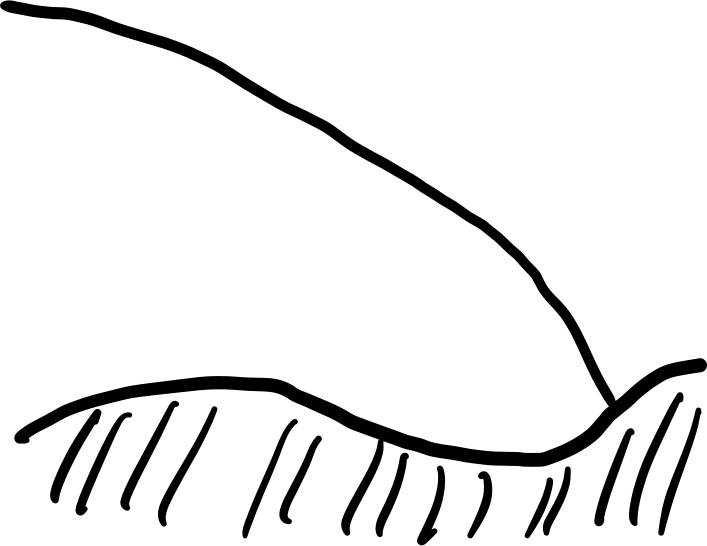
\includegraphics[width=25mm]{figs/wedge.png}} node[xshift=-4mm, yshift=1mm] at (wedge.center) {{\small \emph{ice}}};
  \node[right=of wedge] (unbounded) {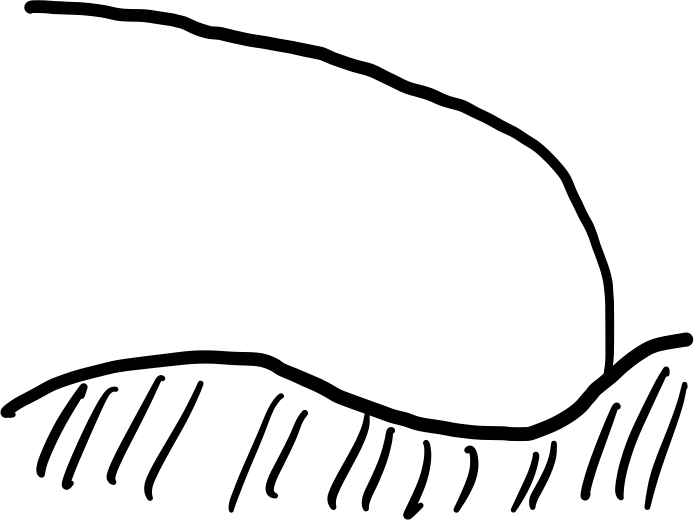
\includegraphics[width=26mm]{figs/unbounded.png}} node[xshift=-2mm, yshift=1mm] at (unbounded.center) {{\small \emph{ice}}};
  \node[right=of unbounded] (realistic) {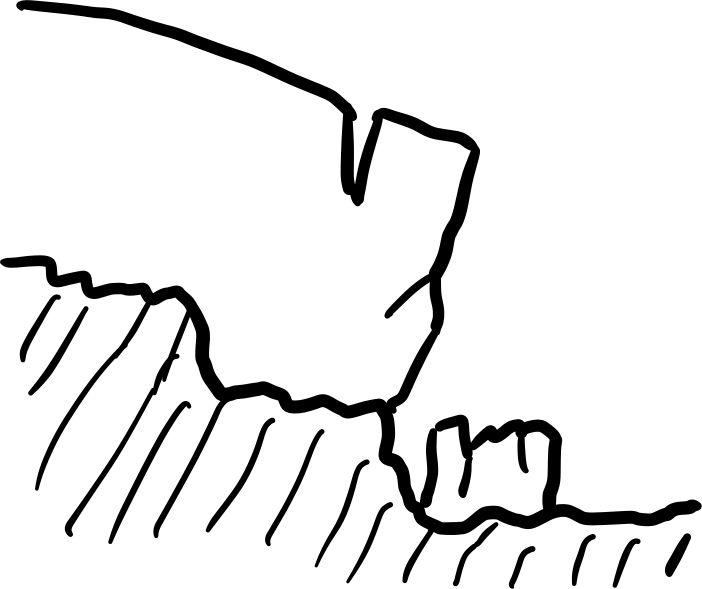
\includegraphics[width=26mm]{figs/realistic.png}} node[xshift=-6mm, yshift=4mm] at (realistic.center) {{\small \emph{ice}}};
\end{tikzpicture}
\end{center}

\vspace{-2mm}

\caption{Glacier margins with finite-slope ``wedge'' shapes (left) are possible, while shallow theory has fractional powers (center).  Actual glacier margins might have overhangs and fractures (right).}
\label{fig:margins}
\end{figure}

Major numerical models all ignore overhangs \cite{IsaacStadlerGhattas2015,Jouvetetal2008,LofgrenAhlkronaHelanow2022,WirbelJarosch2020},
and fractures do not occur within the viscous-fluid physics of such models, and likewise within the current work.  Future models might allow fractures, supplementing momentum conservation with an advected damage variable and a stress-failure criterion \cite{PralongFunk2005}.  Averaged over hundred-meter scale, the emergent margin shapes might suggest a regularity assumption and Sobolev space for surface elevations in the viscous theory.

We attempt to choose $\cX$ based on mathematical considerations within the viscous theory.  First, well-posedness of the fixed-domain Stokes problem \eqref{eq:glenstokes:weak}, along with the surface trace bound in Lemma  \ref{lem:surfacetracebound}, generates a well-defined map from an admissible surface elevation $s\in \cK$ to the surface motion term $\bu|_s\cdot \bn_s$ appearing in \eqref{eq:be:viearly}.  To properly understand this map we change domain notation.  For an implicit time step, the ice domain depends only on the surface elevation, so we write
\begin{equation}
\boxed{\Lambda(s) = \left\{(x,z)\,:\,b(x) < z < s(x)\right\} \subset \Omega \times \RR.} \label{eq:domainfroms}
\end{equation}
(This replaces the time-dependent notation in \eqref{eq:icydomain}.)  For a given input surface $s$, the proposed map first solves the Stokes model \eqref{eq:glenstokes:weak} over $\Lambda(s)$, then evaluates the trace of $\bu$ along $\Gamma_s$, then extends by zero \eqref{eq:defineus}, and finally multiplies by $\bn_s$.  For this to be defined $s\in\cK\subset\cX$ must be sufficiently-regular, and for the space $\cX$ we will propose $W^{1,\rr}(\Omega)$ because of the next Lemma.  Let $[L]>0$ be a representative \emph{horizontal} scale for $\Omega\subset\RR^2$, and then for $\omega\in W^{1,\rr}(\Omega)$ define the norm
\begin{equation}
\|\omega\|_{W^{1,\rr}} = \left(\int_\Omega |\omega|^\rr\,dx + [L]^\rr \int_\Omega |\grad \omega|^\rr\,dx\right)^{1/\rr}; \label{eq:norm:Omega}
\end{equation}
compare \eqref{eq:vnorm}.  We now show that if $s\in W^{1,\rr}(\Omega)$ then the measurable function $\bu|_s\cdot \bn_s$ is in the dual space $(W^{1,\rr}(\Omega))'$.

\begin{lemma}[Bound on surface motion] \label{lem:phibound}  Suppose $2 \le \rr \le \infty$ and that $s\in W^{1,\rr}(\Omega)$ satisfies $s\ge b$ and $s=b$ on $\partial\Omega$.  Then there is a constant $C(\|s\|_{W^{1,\rr}})>0$ so that for all  $\omega\in W^{1,\rr}(\Omega)$,
\begin{equation}
\left|\int_\Omega \bu|_s\cdot \bn_s \,\omega\,dx\right| \le C(\|s\|_{W^{1,\rr}})\, \|\omega\|_{W^{1,\rr}}. \label{eq:phibound:early}
\end{equation}
\end{lemma}

\begin{proof}  Recall that $dS = |\bn_s|\,dx = \sqrt{1+|\grad s|^2}\,dx$ is the surface area element for $\Gamma_s \subset \partial \Lambda$.  Apply H\"older's inequalities:
\begin{align}
\Big|\int_\Omega \bu|_s\cdot \bn_s \, &\omega\,dx\Big| \le \int_\Omega \big|\bu|_s\big| |\bn_s|^{1/\pp} |\bn_s|^{1/\pp'} |\omega|\,dx \label{eq:phibound:zero} \\
    &\le \left(\int_\Omega \big|\bu|_s\big|^\pp |\bn_s|\,dx\right)^{1/\pp} \left(\int_\Omega |\bn_s| |\omega|^{\pp'} \,dx\right)^{1/\pp'} \notag \\
    &\le \left(\int_{\Gamma_s} |\bu|^\pp \,dS\right)^{1/\pp} \left(\int_\Omega |\bn_s|^\rr \,dx\right)^{1/(\pp'\rr)} \left(\int_\Omega |\omega|^{\pp'\rr'} \,dx\right)^{1/(\pp'\rr')}. \notag
\end{align}
From bound \eqref{eq:surfacetracebound} we may write
\begin{equation}
\left|\int_\Omega \bu|_s\cdot \bn_s \, \omega\,dx\right| \le C \left(\int_\Omega \left(1+|\grad s|^2\right)^{\rr/2}\,dx\right)^{1/(\pp'\rr)} \|\omega\|_{L^{\pp'\rr'}}.
\end{equation}
Note that if $\alpha\ge 0$ then $(1+\alpha)^{\rr/2} \le 2^{(\rr-2)/2} (1+\alpha^{\rr/2})$, so, using generic constants,
\begin{align}
\left|\int_\Omega \bu|_s\cdot \bn_s \, \omega\,dx\right| &\le C \left(2^{(\rr-2)/2} \int_\Omega 1 + |\grad s|^\rr\,dx\right)^{1/(\pp'\rr)} \|\omega\|_{L^{\pp'\rr'}} \label{eq:phibound:one} \\
  &\le C \left(|\Omega| + [L]^{-\rr}\|s\|_{W^{1,\rr}}^\rr\right)^{1/(\pp'\rr)} \|\omega\|_{L^{\pp'\rr'}}. \notag
\end{align}
Since $2 \le \pp' \le \pp'\rr' < \infty$, by Sobolev's inequality, e.g.~Theorem 8.8 from \cite{LiebLoss1997} using $n=2$, $k=m=1$, $p=\rr$, and $\omega=\pp'\rr'$, we have $\|\omega\|_{L^{\pp'\rr'}} \le C \|\omega\|_{W^{1,\rr}}$, thus \eqref{eq:phibound:early}.
\end{proof}

Because $\Omega\subset \RR^2$, if additionally $\rr>2$ then $W^{1,\rr}(\Omega) \hookrightarrow C(\bar\Omega)$.  Note that in Section \ref{sec:application} the FE approximation $s_h\approx s$ will be continuous and piecewise-linear.  Thus for $2 < \rr \le \infty$ we define from now on
\begin{equation}
\boxed{\cX = W^{1,\rr}(\Omega).} \label{eq:defineX}
\end{equation}
The admissible subset $\cK \subset \cX$ for surface elevations is defined by \eqref{eq:be:admissible}.  By Lemma \ref{lem:surfacetracebound} the surface velocity $\bu|_s$ is well-defined as a measurable function, and its $L^\pp(\Gamma_s)$ norm is bounded.  By Lemma \ref{lem:phibound} the surface motion term $\bu|_s\cdot\bn_s$ is in $\cX'$.

However, to proceed we must conjecture that a norm of $\bu|_s$ is Lipschitz as a function of $s$.  Proving this apparently requires additional, detailed knowledge about Stokes problem \eqref{eq:glenstokes:weak}.  The dependence of scalar Laplacian-type equations on the domain is addressed in some literature, for example \cite{Daners2003}, but such results for Stokes problems are not known to this author.

\begin{conjecture}[Surface velocity is Lipschitz in the surface elevation] \label{conj:lipschitz}
There exists $2 < \rr \le \infty$ so that if $R>0$ then there is $C(R)>0$ so that for $\sigma,s\in B_R \cap \cK = \{t\in \cK\,:\,\|t\|_{\cX} \le R\}$ we have
\begin{equation}
\big\|\bu|_\sigma - \bu|_s\big\|_{L^{\rr'}} \le C(R) \|\sigma-s\|_{\cX} \label{eq:ulipschitz}
\end{equation}
\end{conjecture}

From now on we will assume that Conjecture \ref{conj:lipschitz} holds for some $\rr>2$, and we define the nonlinear \emph{surface motion map} $\Phi:\cK \to \cX'$ by
\begin{equation}
\boxed{\Phi(s)[\omega] = -\int_\Omega \bu|_s\cdot\bn_s\,\omega\,dx,} \label{eq:definePhi}
\end{equation}
for $\omega\in \cX$.  Unsurprisingly the Conjecture implies that this map is Lipschitz, but this requires proof.

\begin{definition} \label{def:lipshitz}
For $R>0$ let $B_R = \{v\in \cX\,:\,\|v\|\le R\}$.  We say that a map $f:\cK \to \cX'$ is \emph{Lipshitz on bounded subsets of $\cK$} if for every $R>0$ there is $C(R)>0$ so that
\begin{equation}
\|f(v)-f(w)\|_{\cX'} \le C(R) \|v-w\|_{\cX} \quad \text{ for all } v,w \in B_R \cap \cK.  \label{eq:liponbounded}
\end{equation}
\end{definition}

\begin{lemma} \label{lem:philipschitz}  The map $\Phi$ is Lipschitz on bounded subsets of $\cK$.
\end{lemma}

\begin{proof}  Assume without loss of generality that $R\ge \|b\|_\cX$, so $b\in B_R \cap \cK$.  Suppose $\sigma,s\in B_R \cap \cK$.  For any $\omega\in\cX$, in the following we add and subtract $\bu|_s \cdot \bn_\sigma$, and use the triangle inequality $|\bn_\sigma|=\left(1+|\grad \sigma|^2\right)^{1/2} \le 1 + |\grad \sigma|$:
\begin{align}
\Big|\Phi(\sigma)[\omega] - \Phi(s)[\omega]\Big| &\le \int_\Omega \Big|\bu|_\sigma - \bu|_s\Big| |\bn_\sigma| |\omega|\,dx + \int_\Omega \big|\bu|_s\big| |\bn_\sigma-\bn_s| |\omega|\,dx \\
    &\le \int_\Omega \Big|\bu|_\sigma - \bu|_s\Big| |\omega|\,dx + \int_\Omega \Big|\bu|_\sigma - \bu|_s\Big| |\grad \sigma| |\omega|\,dx \notag \\
    &\qquad\qquad + \int_\Omega \big|\bu|_s\big| |\grad \sigma-\grad s| |\omega|\,dx \notag
\end{align}
By applying H\"older's inequality to each of these integrals we have
\begin{align}
\int_\Omega \Big|\bu|_\sigma - \bu|_s\Big| |\omega|\,dx &\le \big\|\bu|_\sigma - \bu|_s\big\|_{L^{\rr'}} \|\omega\|_{L^{\rr}} \le \|\bu|_\sigma - \bu|_s\|_{L^{\rr'}} \|\omega\|_{\cX}, \label{eq:philipschitz:1} \\
\int_\Omega \Big|\bu|_\sigma - \bu|_s\Big| |\grad \sigma| |\omega|\,dx &\le \left(\int_\Omega \Big|\bu|_\sigma - \bu|_s\Big|^{\rr'} |\omega|^{\rr'}\, dx\right)^{1/\rr'} \|\grad \sigma\|_{L^\rr} \label{eq:philipschitz:2} \\
    &\le [L]^{-1} \big\|\bu|_\sigma - \bu|_s\big\|_{L^{\rr'}} \|\sigma\|_{\cX} \|\omega\|_{L^\infty}, \notag \\
\int_\Omega \big|\bu|_s\big| |\grad \sigma-\grad s| |\omega|\,dx &\le \left(\int_\Omega \big|\bu|_s\big|^{\rr'} |\omega|^{\rr'}\, dx\right)^{1/\rr'} \|\grad \sigma- \grad s\|_{L^\rr}  \label{eq:philipschitz:3} \\
    &\le [L]^{-1} \big\|\bu|_s - \bzero\big\|_{L^{\rr'}} \|\sigma-s\|_{\cX} \|\omega\|_{L^\infty}. \notag
\end{align}
Note that $\bu|_b=\bzero$; there is no flow when there is no glacier.  Because $\rr>2$, Sobolev's inequality gives $\|\omega\|_{L^\infty} \le c_\infty \|\omega\|_\cX$ for some $c_\infty>0$.  Now apply Conjecture \ref{conj:lipschitz} to each of \eqref{eq:philipschitz:1}--\eqref{eq:philipschitz:3}:
\begin{equation}
\big|\Phi(\sigma)[\omega] - \Phi(s)[\omega]\big| \le \tilde C(R) \left(1 + c_\infty [L]^{-1} \left(\|\sigma\|_{\cX} + \|s - b\|_{\cX}\right)\right) \|\sigma-s\|_{\cX} \|\omega\|_{\cX}.
\end{equation}
Recalling that $b\in B_R\cap \cK$, use the triangle inequality again to conclude with $C(R) = \tilde C(R) \left(1 + 3 c_\infty [L]^{-1} R\right)$.
\end{proof}

At this point we have the tools needed to make the continuum free-boundary model for a backward-Euler time-step \eqref{eq:be:ske} mathematically precise.

\begin{definition} For $\Delta t>0$, $s\in\cK$, and $\omega\in\cX$ define the nonlinear (Stokes) \emph{geometry update operator} $F_{\Delta t}:\cK\to\cX'$ as
\begin{equation}
\boxed{F_{\Delta t}(s)[\omega] = \Delta t\,\Phi(s)[\omega] + \int_\Omega s \omega.}  \label{eq:be:Fdefine}
\end{equation}
Assume that $\ell^n$, defined from data by \eqref{eq:be:source}, is in $\cX'$.  We say that the surface elevation $s=s^n \in \cK$ solves the (weak-form) \emph{implicit time-step problem} if
\begin{equation}
\boxed{F_{\Delta t}(s)[\sigma-s] \ge \ell^n[\sigma-s] \quad \text{for all } \sigma \in \cK.} \label{eq:be:vi}
\end{equation}
\end{definition}

If Conjecture \ref{conj:lipschitz} holds then $\Phi$ and thus $F_{\Delta t}$ are well-defined and Lipschitz on bounded subsets.  The reader should confirm that the weak-form VI \eqref{eq:be:vi} then merely rewrites \eqref{eq:be:viearly}.  This VI is the precise version and meaning of strong-form NCP \eqref{eq:be:ncp}.

The seven boxed definitions and inequalities above, namely \eqref{eq:be:source}, \eqref{eq:be:admissible}, \eqref{eq:domainfroms}, \eqref{eq:defineX}, \eqref{eq:definePhi}, \eqref{eq:be:Fdefine}, and \eqref{eq:be:vi}, form a continuum model for a single time-step of glacier evolution based on Stokes dynamics.  Although Conjecture \ref{conj:lipschitz} is used in the construction of the operator $F_{\Delta t}$, this model is precise enough to be mathematically analyzed, and a future existence and/or uniqueness result for \eqref{eq:be:vi} is possible.  However, we will regularize the model in the next Section, and, based on numerical evidence, well-posedness for this regularization is credible.  Sections \ref{sec:abstractestimate} and \ref{sec:application} then prove an error estimation theorem for an FE approximation of the regularized model.


\section{Conjectural well-posedness for the regularized problem} \label{sec:conjectural}

Theorem \ref{thm:glacierapp}, our main result to come, is numerical.  It bounds the FE error in surface elevation by extending an abstract technique from Falk \cite{Falk1974} to a large class of nonlinear operators.  It is tied to the concepts of monotonicity \cite{Minty1963} and coercivity \cite[Chapter III]{KinderlehrerStampacchia1980}.

\begin{definition} \label{def:monotonecoercive}
Suppose $\cX$ is a Banach space, with norm $\|\cdot\|$, and $\cK\subset \cX$ is closed and convex.  An operator $f:\cK \to \cX'$ is said to be \emph{monotone} if
\begin{equation}
\left(f(v)-f(w)\right)[v-w] \ge 0 \qquad \text{for all } v,w \in \cK, \label{eq:monotone}
\end{equation}
and \emph{strictly monotone} if in addition equality implies $v=w$.  It is \emph{coercive} if there is $w\in \cK$ so that $\left(f(v)-f(w)\right)[v-w]/\|v-w\| \to +\infty$ for $v \in \cK$ as $\|v\| \to +\infty$.  It is \emph{$\qq$-coercive} \emph{\cite{Bueler2021conservation}} for $\qq>1$ if there exists $\alpha>0$ such that
\begin{equation}
\left(f(v)-f(w)\right)[v-w] \ge \alpha \|v-w\|^\qq \qquad \text{for all } v,w \in \cK. \label{eq:qcoercive}
\end{equation}
\end{definition}

Note that $\qq$-coercivity implies coercivity and strict monotonicity.  Also, $2$-coercivity is sometimes called \emph{strong monotonicity} \cite{Chow1989}.

Theorem \ref{thm:abstractestimate} in the next section applies to VIs for operators $f:\cK\to\cX'$ which are $\qq$-coercive.  We would want to apply the Theorem to $F_{\Delta t}$ \eqref{eq:be:Fdefine} acting on an admissible subset $\cK$ of $\cX=W^{1,\rr}(\Omega)$, and note that the surface motion map $\Phi$ \eqref{eq:definePhi} is the main term in $F_{\Delta t}$.  However, apparently-new examples in Appendix \ref{app:noncoercive} show that $\Phi$ is not $\qq$-coercive or strictly monotone over $W^{1,\rr}(\Omega)$ for any $\rr$.  These examples can be constructed for any bedrock $b$ possessing local minima, by filling with flat ice.\footnote{The same examples negatively resolve a previously open question of uniqueness, for elevation-independent SMB, in the shallow ice approximation.  See Appendix \ref{app:noncoercive}.}  Since $F_{\Delta t}$ adds the integral $\int_\Omega s\omega$ to the surface motion term $\Delta t\,\Phi(s)[\omega]$, lack of coercivity for $\Phi$ does not dis-prove it for $F_{\Delta t}$, but we proceed in another direction.

The numerical experiments in Appendix \ref{app:numerical} turn out to show that the surface motion operator $\Phi$ is \emph{nearly} $\qq$-coercive.  In these experiments thousands of high-resolution surface pairs $\sigma,s\in \cK\subset W^{1,\rr}(\Omega)$ were generated from a 1D glacier simulation.  Coercivity ratios were computed for exponents $\rr=\qq=4$:
\begin{equation}
\frac{(\Phi(\sigma) - \Phi(s))[\sigma - s]}{\|\sigma-s\|_{W^{1,4}}^{4}}. \label{eq:ratios}
\end{equation}
Surface velocities from the Stokes model were used when evaluating \eqref{eq:definePhi}.  Recalling Definition \eqref{def:monotonecoercive}, if $\Phi$ were $4$-coercive over $\cX=W^{1,4}(\Omega)$, and if all computations were exact, then these ratios would all exceed a coercivity constant $\alpha>0$.  Though standard presentations of Stokes models for glaciers give no reason to expect these ratios to even be non-negative, Appendix \ref{app:numerical} shows that under mesh refinement the pairs yielding negative ratios become quite rare.  The mean and median ratios are decidely positive, and under refinement they stabilize away from zero.

\newcommand{\wSIA}{\tilde w}
However, because Appendix \ref{app:noncoercive} examples show that $\Phi$ is not actually $\qq$-coercive over $W^{1,\rr}(\Omega)$, we will regularize the surface motion term using the shallow theory of ice \cite{GreveBlatter2009}.  In the limit of small aspect ratios this isothermal shallow ice approximation theory yields an expression for the surface vertical motion:
% Gamma = \frac{\nn+1}{\nn+2} 2 (rho g)^2 / (\nn+2),  i.e. (n+1)/(n+2) times the usual Gamma
\begin{equation} \label{eq:verticalvelocitysia}
\wSIA|_s = \Div \left(\Gamma (s-b)^{\nn+1} |\grad s|^{\nn-1} \grad s\right).
\end{equation}
Here $\nn$ is Glen's exponent and $\Gamma>0$ is a softness constant computable from the viscosity scale $\nu_\pp$ in \eqref{eq:glen}.

Formula \eqref{eq:verticalvelocitysia} degenerates at the glacier margin where the thickness $s-b$ goes to zero, so we regularize using a fixed ice thickness $H_0>0$.  Let $\nn=3$ and $\eps>0$.  Writing the Stokes velocity in components $\bu = (u_1,u_2,w)$, for $\omega \in \cX$ we define this regularized version of weak formula \eqref{eq:definePhi}:
\begin{equation} \label{eq:defineregularizedPhi}
\Phi^\eps(s)[\omega] = \int_\Omega \Big(\big(u_1|_s,u_2|_s\big) \cdot \grad s - (1-\eps) w|_s\Big) \omega + \eps\, \Gamma H_0^4 |\grad s|^2 \grad s \cdot \grad \omega.
\end{equation}
This formula replaces the Stokes vertical velocity $w|_s$ with the convex combination $(1-\eps)w|_s + \eps\, \wSIA|_s$.  If $\Phi$ is Lipschitz on bounded subsets of $\cK$ (Lemma \ref{lem:philipschitz}) then so is $\Phi^\eps$; inequality (3.4) in \cite{JouvetBueler2012} proves this.  Regularization \eqref{eq:defineregularizedPhi} is likely to generate a $4$-coercive operator over $W^{1,4}(\Omega)$ because of properties of the (weak-form) $\pp$-Laplacian operator \cite[for example]{ChoeLewis1991}.  The $\eps$ term in \eqref{eq:defineregularizedPhi} is a multiple of the $4$-Laplacian of $s$, namely $-\Div(|\grad s|^2 \grad s)$, which is $4$-coercive over $W^{1,4}(\Omega)$.

The numerical experiments in Appendix \ref{app:numerical} used values $\eps=0.1$ and $H_0=1000$ meters in \eqref{eq:defineregularizedPhi}.  The observed effect was that negative coercivity ratios \eqref{eq:ratios} disappeared at high spatial resolution, and that the experimental distribution of ratios was bounded away from zero.  However, we are not able to \emph{prove} that $\Phi^\eps$ in \eqref{eq:defineregularizedPhi} is $4$-coercive.  A proof would seem to depend on novel and nontrivial insights into the glaciological Stokes problem.  The numerical analysis in Section \ref{sec:application} will therefore be based on the following final conjecture.

\begin{conjecture}[Regularized surface motion $\Phi^\eps(s)$ is $4$-coercive over admissible surface elevations in $W^{1,4}$] \label{conj:regcoercive}  Suppose Conjecture \ref{conj:lipschitz} holds for $\rr=4$, and let $\cX = W^{1,4}(\Omega)$.  Fix $b\in C^1(\bar\Omega)$ and let $\cK=\{\sigma\in\cX\,:\,\sigma\ge b \text{ and } \sigma|_{\partial\Omega}=b|_{\partial\Omega}\}$.  There exists $\eps \in (0,1)$ and $H_0>0$, and $\alpha>0$, so that
\begin{equation}
\left(\Phi^\eps(\sigma) - \Phi^\eps(s)\right)[\sigma-s] \ge \alpha \|\sigma-s\|_{\cX}^4 \qquad \text{for all } \sigma,s\in\cK. \label{eq:regcoercive}
\end{equation}
\end{conjecture}

To complete this Section we prove that this Conjecture suffices for well-posedness of the regularized VI problem; recall \eqref{eq:be:Fdefine} and \eqref{eq:be:vi} for the unregularized problem.

\begin{theorem} \label{thm:regularizedwellposed}  Assume Conjectures \ref{conj:lipschitz} and \ref{conj:regcoercive} hold.  Suppose that $s^{n-1}\in\cK$ and define the source term $\ell^n \in \cX'$ as in \eqref{eq:be:source}.  For $\Delta t>0$ define
\begin{equation}
F^\eps_{\Delta t}(s)[\omega] = \Delta t\,\Phi^\eps(s)[\omega] + \int_\Omega s \omega, \label{eq:regularizedF}
\end{equation}
the regularized update operator.  This operator is Lipschitz on bounded subsets and $4$-coercive, thus there exists a unique surface elevation $s\in\cK$ satisfying the VI problem
\begin{equation}
F^\eps_{\Delta t}(s)[\sigma-s] \ge \ell^n[\sigma-s] \quad \text{for all } \sigma \in \cK. \label{eq:regularizedvi}
\end{equation}
\end{theorem}

\begin{proof}  The Lipschitz and $4$-coercive properties are straightforward inequalities following from the Conjectures.  In particular, $F^\eps_{\Delta t}$ is $4$-coercive over $\cK$ with constant $\alpha\Delta t>0$, and thus it is also coercive and strictly-monotone (Definition \ref{def:monotonecoercive}).  Corollary III.1.8 of \cite{KinderlehrerStampacchia1980} now shows unique existence for \eqref{eq:regularizedvi}.
\end{proof}

Theorem \ref{thm:regularizedwellposed} addresses only the well-posedness of a single time-step, over $[t_{n-1},t_n]$.  Its conclusion is certainly not sufficient to show well-posedness of the time-dependent VI problem corresponding to NCP \eqref{eq:ncp}, nor to show that implicit steps converge in the $\Delta t\to 0$ limit.  However, it is a first mathematical step in these directions.  Time-stepping numerical models for the evolution of glacier geometry, using Stokes dynamics, are already in common use.  Their designers apparently expect that each time-step problem, implicit or not, is well-posed, and they believe that computed surface elevations will converge to continuum solutions in some well-behaved manner.


\section{Abstract error estimate for finite element approximation of VIs} \label{sec:abstractestimate}

In this Section we consider the FE approximation of an abstract VI problem in a Banach space.  We will return to glaciological problem \eqref{eq:regularizedvi} in Section \ref{sec:application}.

Let $\cX$ be a real, reflexive Banach space with norm $\|\cdot\|$ and topological dual space $\cX'$.  Denote the dual pairing of $\ell \in \cX'$ and $v\in\cX$ by $\ell[v]$, and define $\|\ell\|_{\cX'} = \sup_{\|v\|=1} \big|\ell[v]\big|$.  Let $\cK \subset \cX$ be a nonempty, closed, and convex subset, the constraint or admissible set.  For a continuous and (generally) nonlinear operator $f:\cK \to \cX'$, and a source functional $\ell\in \cX'$, the abstract VI problem is to find $u\in \cK$ such that
\begin{equation}
f(u)[v-u] \ge \ell[v-u] \quad \text{for all } v\in \cK. \label{eq:vi}
\end{equation}
While \eqref{eq:regularizedvi} is of course in this form, the best known example of \eqref{eq:vi} is the obstacle problem for the Laplacian operator; see \cite{Ciarlet2002,Evans2010,KinderlehrerStampacchia1980} for theory and FE analysis.

If $f:\cK \to \cX'$ is monotone and coercive (Definition \ref{def:monotonecoercive}), and continuous on finite-dimensional subspaces, then problem \eqref{eq:vi} has a solution \cite[Corollary III.1.8]{KinderlehrerStampacchia1980}.  If $f$ is strictly monotone then the solution is unique, and if $f$ is $\qq$-coercive then it coercive and strictly monotone.  On the other hand, if $f$ is Lipschitz on bounded subsets (Definition \ref{def:lipshitz}) then it is continuous.  Recall that $f(u)-\ell \in \cX'$ is generally nonzero if $u$ solves \eqref{eq:vi}, but $f(u)-\ell=0$ when $u$ is in the interior of $\cK$.  Under sufficient regularity assumptions, an NCP strong form generally follows from \eqref{eq:vi}.

Suppose $\cX_h \subset \cX$ is a finite-dimensional subspace, typically some FE space of continuous, piecewise-polynomial functions defined on a mesh.  Let $\cK_h\subset \cX_h$ be a closed and convex subset, and suppose $f_h:\cK_h\to\cX'$ is an approximation of $f$.  Generally $\cK_h \nsubset \cK$---we will not assume that FE states are continuum admissible---and $f_h\ne f$ because of quadrature and other approximations.  In fact, in the standard FE construction of a Stokes-type glacier geometry problem (Section \ref{sec:application}), both $\cK_h \nsubset \cK$ and $f_h\ne f$ apply for practical reasons.

The FE method for \eqref{eq:vi} is the finite-dimensional VI problem
\begin{equation}
f_h(u_h)[v_h-u_h] \ge \ell[v_h-u_h] \quad \text{for all } v_h\in \cK_h. \label{eq:fe:vi}
\end{equation}
We will assume that this problem has a solution $u_h\in\cK_h$, but it need not be unique for the bound \eqref{eq:abstractestimate} below to apply.

The following \emph{a priori} estimation theorem extends the well-known result of Falk \cite{Falk1974}; see also Theorem 5.1.1 in \cite{Ciarlet2002}.  We assume here that $f$ is coercive and Lipschitz on an (unnamed) larger set than $\cK$, which contains the FE solution $u_h$, a technical assumption permiting a clean and general result.  However, we do \emph{not} assume any of the following: $\cK_h \subset \cK$, $f$ is linear, $f_h=f$, $f_h$ is continuous, or $f_h$ is $\qq$-coercive.

\begin{theorem} \label{thm:abstractestimate}  Suppose $u\in\cK$ solves \eqref{eq:vi} and $u_h\in\cK_h$ solves \eqref{eq:fe:vi}.  For $\qq>1$, with conjugate exponent $\qq'=\qq/(\qq-1)$, assume that $f$ is $\qq$-coercive, with constant $\alpha>0$, on a set which contains $\cK$ and the numerical solution $u_h$.  Also, assume $f$ is Lipschitz on bounded subsets of this set.  Let $R_h=\max\{\|u\|,\|u_h\|\}$.  Then there is a constant $c(R_h,\alpha)>0$, not otherwise depending on $u$ or $u_h$, so that
\begin{align}
\|u-u_h\|^\qq &\le \frac{2}{\alpha} \left(\inf_{v\in\cK} \left(f(u)-\ell\right)[v-u_h] + \inf_{v_h\in\cK_h} \left(f(u)-\ell\right)[v_h-u]\right)\label{eq:abstractestimate} \\
   &\quad\, + \frac{2}{\alpha} \left(f(u_h)-f_h(u_h)\right)[u_h] + c(R_h,\alpha) \inf_{v_h\in\cK_h} \|v_h - u\|^{\qq'}. \notag
\end{align}
\end{theorem}

\begin{proof}  It follows from $\qq$-coercivity of $f$ that
\begin{align}
\alpha \|u-u_h\|^\qq &\le \left(f(u)-f(u_h)\right)[u-u_h] \notag \\
  &= f(u)[u] + f(u_h)[u_h] - f(u)[u_h] - f(u_h)[u] \notag \\
  &= f(u)[u] + f_h(u_h)[u_h] - f(u)[u_h] - f(u_h)[u] + \left(f(u_h)-f_h(u_h)\right)[u_h]. \label{eq:abstract:one}
\end{align}
Next, for arbitrary $v\in\cK$ and $v_h\in\cK_h$, rewrite \eqref{eq:vi} as $f(u)[u]     \le f(u)[v] + \ell[u-v]$ and \eqref{eq:fe:vi} as $f_h(u_h)[u_h] \le f_h(u_h)[v_h] + \ell[u_h-v_h]$.  Then
\begin{align}
\alpha \|u-u_h\|^\qq &\le f(u)[v] + \ell[u-v] + f(u_h)[v_h] + \ell[u_h-v_h] \label{eq:abstract:two} \\
  &\qquad - f(u)[u_h] - f(u_h)[u] + \left(f(u_h)-f_h(u_h)\right)[u_h] \notag \\
  &= \left(f(u)-\ell\right)[v-u_h] + \left(f(u)-\ell\right)[v_h-u] \notag \\
  &\qquad + \left(f(u)-f(u_h)\right)[u-v_h] + \left(f(u_h)-f_h(u_h)\right)[u_h] \notag
\end{align}
Since $u,u_h\in B_{R_h}$, by the Lipschitz assumption there is $C(R_h)>0$ so that
\begin{equation}
\left(f(u)-f(u_h)\right)[u-v_h] \le C(R_h) \|u-u_h\|\|u-v_h\|. \label{eq:abstract:three}
\end{equation}
Noting $1<\qq<\infty$, use Young's inequality with $\eps>0$ \cite[Appendix B.2]{Evans2010} on \eqref{eq:abstract:three}:
\begin{align}
\alpha \|u-u_h\|^\qq &\le \left(f(u)-\ell\right)[v-u_h] + \left(f(u)-\ell\right)[v_h-u]  \label{eq:abstract:four} \\
  &\qquad + C(R_h) \left(\eps\|u-u_h\|^\qq + \tilde C(\eps) \|u-v_h\|^{\qq'}\right) \notag \\
  &\qquad + \left(f(u_h)-f_h(u_h)\right)[u_h], \notag
\end{align}
where $\tilde C(\eps) = (\eps \qq)^{-\qq'/\qq} {\qq'}^{-1}$.  Choose $\eps>0$ so that $C(R_h) \eps \le \alpha/2$, and subtract:
\begin{align}
\frac{\alpha}{2} \|u-u_h\|^\qq &\le \left(f(u)-\ell\right)[v-u_h] + \left(f(u)-\ell\right)[v_h-u]  \label{eq:abstract:five} \\
  &\qquad + C(R_h) \tilde C(\eps) \|u-v_h\|^{\qq'} + \left(f(u_h)-f_h(u_h)\right)[u_h] \notag
\end{align}
Take infimums to show \eqref{eq:abstractestimate}.
\end{proof}

Considering the residual $f(u)-\ell\in \cX'$ for a unilateral obstacle problem, over $\Omega\subset \RR^d$, allows us to refine the estimate.  In this case the residual is a positive measure $d\mu_u$ supported in the active set $A_u\subset \Omega$ \cite[Theorem II.6.9]{KinderlehrerStampacchia1980}.  The first two terms in bound \eqref{eq:abstractestimate} represent errors made within $A_u$.

\begin{corollary}  \label{cor:abstractwithmeasure}  Suppose $\cX=W^{1,\rr}(\Omega)$, a space of scalar functions, over a domain $\Omega\subset\RR^d$, and suppose $\cK\subset\cX$ is defined as in \eqref{eq:be:admissible} for an obstacle $b$.  Let $d\mu_u = f(u)-\ell$, and define the active set $A_u=\{x\in\Omega\,:\,u(x)>b(x)\}$.  Under the assumptions of Theorem \ref{thm:abstractestimate} we have the bound
\begin{align}
\|u-u_h\|^\qq &\le \frac{2}{\alpha} \left(\inf_{v\in\cK} \int_{A_u} v - u_h\,d\mu_u + \inf_{v_h\in\cK_h} \int_{A_u} v_h - b\,d\mu_u\right)
  \label{eq:abstractwithmeasure} \\
   &\quad\, + \frac{2}{\alpha} \left(f(u_h)-f_h(u_h)\right)[u_h] + c \inf_{v_h\in\cK_h} \|v_h - u\|^{\qq'}. \notag
\end{align}
\end{corollary}

The original result by Falk \cite{Falk1974}, which computes residual norms, loses the active-set information in Corollary \ref{cor:abstractwithmeasure}.  The next Corollary makes this historical connection by applying a norm-based approach; $\cX=W^{1,\rr}(\Omega) \subset L^\qq(\Omega) = \cB$ would be typical.

\begin{corollary}  \label{cor:abstractestimate:Bnorm}  Suppose that $\cX$ continuously and densely embeds into a larger Banach space: $\cX \hookrightarrow \cB$, $\bar{\cX} = \cB$, and $\cB' \subset \cX'$.  Suppose $f:\cK\to\cB'$ and $\ell\in\cB'$.  Under the assumptions of Theorem \ref{thm:abstractestimate} we have
\begin{align}
\|u-u_h\|^\qq &\le \frac{2}{\alpha} \|f(u)-\ell\|_{\cB'} \left( \inf_{v\in\cK} \|v-u_h\|_{\cB} +   \inf_{v_h\in\cK_h} \|v_h-u\|_{\cB} \right) \label{eq:abstractestimate:Bnorm} \\
   &\qquad + \frac{2}{\alpha} \left(f(u_h)-f_h(u_h)\right)[u_h] + c\,\inf_{v_h\in\cK_h} \|v_h - u\|^{\qq'}. \notag
\end{align}
\end{corollary}

The Falk result \cite{Falk1974} is recovered when $\cX, \cB$ are Hilbert spaces, and assuming that $f(v)[w]=f_h(v)[w]=a(v,w)$ is bilinear, uniformly-elliptic, and continuous.\footnote{The definition of uniform ellipticity coincides with definition \eqref{eq:qcoercive} of $2$-coercive, and continuity of $a(v,w)$ implies \eqref{eq:liponbounded}.}  In this context, up to isomorphism, $f(u)-\ell \in \cH$.  Since $f$ is defined on all of $\cX$, the technical assumption about a larger set containing $u_h$ is unnecessary.  With these simplifications, Corollary \ref{cor:abstractestimate:Bnorm} reduces to Theorem 1 in \cite{Falk1974}.

Note that if $u$ is in the interior of $\cK$, and if $f=f_h$, then all bounds \eqref{eq:abstractestimate}, \eqref{eq:abstractwithmeasure}, and \eqref{eq:abstractestimate:Bnorm} reduce to their last error term.  Thus we get Cea's lemma \cite[Theorem 2.4.1]{Ciarlet2002}, but now stated in a Banach space and for a coercive nonlinear operator.  For glaciers this case occurs when the entire domain $\Omega$ is covered by ice.

The ``$\inf_{v\in\cK}$'' terms in bound \eqref{eq:abstractestimate} is generally nonzero when $\cK_h \not\subset \cK$.  To see how this can occur in a unilateral obstacle problem, even for an arbitrarily smooth obstacle, suppose $\cK$ is defined as in \eqref{eq:be:admissible}.  Suppose $b_h=\pi_h b$ is the FE interpolant of $b$, and define $\cK_h=\{v_h \in \cX_h\,:\,v_h\ge b_h \text{ and } v_h|_{\partial\Omega}=b_h|_{\partial\Omega}\}$.  While $b_h(x_j)=b(x_j)$ for the interpolation nodes $x_j$, generally $b_h(x) \ge b(x)$ will not hold for all $x\in\Omega$ (Figure \ref{fig:nonadmissible}; see also \cite[Figure 5.1.3]{Ciarlet2002}).  That is, nodal admissibility does not imply admissibility.

\begin{figure}[ht]
\begin{center}
\begin{tikzpicture}[scale=1.1, domain=0.0:4.0, samples=200]
  \draw[black,thin,->] (-0.3,0.0) -- (4.5,0.0) node [xshift=2mm] {$x$};
  \draw plot (\x, {1.5 + 0.8 * cos(1.8*\x r)});
  \node[yshift=-2mm] at (2.0, 0.7) {$b$};
  \newcommand{\xlist}{0.0, 1.0, 1.4, 2.4, 3.0, 4.0}
  \foreach \x [remember=\x as \lastx] in \xlist {
      \draw (\x, 0.0) circle (1.5pt);
      \filldraw (\x, {1.5 + 0.8 * cos(1.8*\x r)}) circle (1.5pt);
      \draw[dashed] (\lastx, {1.5 + 0.8 * cos(1.8*\lastx r)}) -- (\x, {1.5 + 0.8 * cos(1.8*\x r)});
  }
  \node[yshift=3mm] at (3.0, 0.0) {$x_i$};
  \node[xshift=3mm, yshift=-7mm] at (0.0, 2.3) {$b_h$};
\end{tikzpicture}
 \quad \begin{tikzpicture}[scale=1.1, domain=0.0:4.0, samples=200]
  \draw[black,thin,->] (-0.3,0.0) -- (4.5,0.0) node [xshift=2mm] {$x$};
  \draw plot (\x, {1.5 + 0.8 * cos(1.8*\x r)});
  \newcommand{\xlist}{0.0, 1.0, 1.4, 2.4, 3.0, 4.0}
  \newcommand{\xymaxlist}{0.0/2.3, 1.0/2.3, 1.4/1.3182, 2.4/2.0078, 3.0/2.3, 4.0/2.3}
  \foreach \x/\y in \xymaxlist {
      \draw (\x, 0.0) circle (1.5pt);
      \filldraw (\x, \y) circle (1.5pt);
  }
  \node[yshift=3mm] at (3.0, 0.0) {$x_i$};
  \draw[dashed] (0.0,2.3) -- (1.0,2.3) -- (1.4,1.3182) -- (2.4,2.0078) -- (3.0,2.3) -- (4.0,2.3);
  \node[yshift=-2mm] at (2.0, 0.7) {$\psi$};
  \node[xshift=5mm, yshift=-3mm] at (1.0, 2.3) {$\psi_h$};
\end{tikzpicture}

\end{center}
\caption{Left: If $b_h=\pi_h b$ is the interpolant of $b$ then generally $\cK_h\nsubset\cK$.  Right: Defining $b_h=R_h^{\oplus} b$, using \eqref{eq:monotoneop}, implies $b_h\ge b$ and $\cK_h\subset\cK$.}
\label{fig:nonadmissible}
\end{figure}

For unilateral obstacle problems and $P_1$ or $Q_1$ elements we may force $\cK_h\subset\cK$ by using a monotone restriction operator \cite{BuelerFarrell2024}, defined as follows.  For a node $x_i$ let $N_i$ be the union of elements adjacent to $x_i$.  Define $R_h^{\oplus}b\in\cX_h$ by
\begin{equation}
(R_h^{\oplus}b)(x_i) = \sup_{x \in N_i} b(x). \label{eq:monotoneop}
\end{equation}
If $b_h=R_h^{\oplus} b$ then $b_h(x)\ge b(x)$ for all $x\in \Omega$ (Figure \ref{fig:nonadmissible}; right), thus $\cK_h\subset \cK$ and the ``\,$\inf_{v\in\cK}$'' term vanishes from the bounds.

In summary, Theorem \ref{thm:abstractestimate} is a powerful and nontrivial generalization of Falk's bound \cite{Falk1974} and Cea's lemma.  We now return to the glacier problem.


\section{Application to numerical glacier models} \label{sec:application}

Now we can apply the above theory to a time-step of an evolving-surface, Stokes-based glacier simulation.  Our approach essentially defines the phrase ``conforming FE method'' for such glacier simulations.  We will combine the three major threads from earlier Sections: well-posedness and \emph{a priori} bounds for the glaciological Stokes problem on a fixed domain (Section \ref{sec:stokes}), conjectural $4$-coercivity and well-posedness of the regularized VI problem for an implicit and fully-coupled step of the surface elevation (Sections \ref{sec:model} and \ref{sec:conjectural}), and an abstract error estimate for the FE solutions of such VIs (Section \ref{sec:abstractestimate}).

Practical models for glaciers, generally based on unstructured meshes in the 2D map-plane, use polygonal domain geometry for the 3D Stokes problem \cite{Brinkerhoff2023,IsaacStadlerGhattas2015,Jouvetetal2008,Lengetal2012}.  For this reason we assume that the domain $\Omega \subset \RR^2$ is a polygon, and that the discrete bed and surface elevations $b_h,s_h$ are from the continuous $P_1$ FE space $\cX_h$ over a triangulation $\cT_h$ of $\Omega$ (Figure \ref{fig:fe:domain}).  The 3D mesh need not be extruded vertically from $\cT_h$, as shown in Figure \ref{fig:fe:domain}, but this is a possibility.

\begin{figure}[ht]
\begin{center}
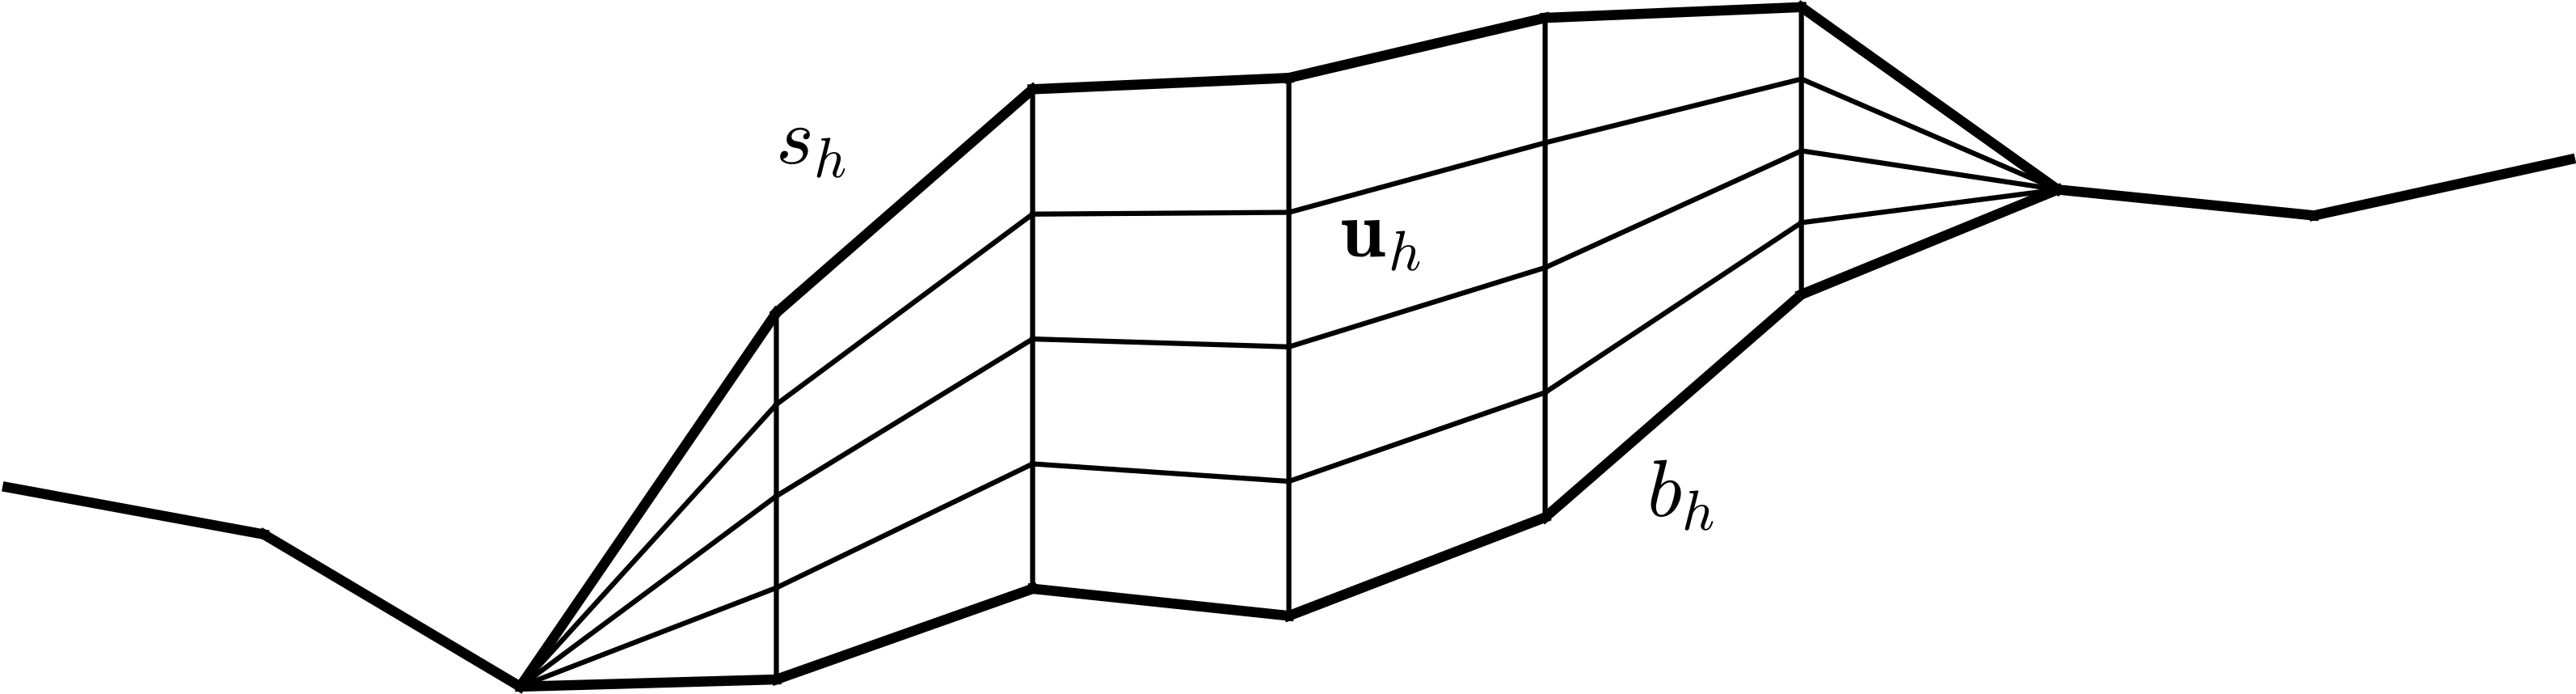
\includegraphics[width=0.7\textwidth]{genfigs/extruded.pdf}
\end{center}
\caption{The Stokes problem for the velocity $\bu_h$ is solved on a polygonal domain, on a mesh between $P_1$ functions $b_h$ and $s_h$.  Computation of $F_{\Delta t}^h$ requires evaluation of the surface trace $\bu_h|_{s_h}$.}
\label{fig:fe:domain}
\end{figure}

We will assume that the original bed elevation $b$ is well-behaved, $b\in C^1(\bar\Omega)$.  In practice $b$ is provided via a high resolution map derived from ice-penetrating radar \cite{Morlighemetal2017}, often over a much finer mesh than $\cT_h$.  For the discrete bed $b_h\in\cT_h$ we suppose $b_h=b$ along $\partial\Omega$.  By application of monotone restriction, thus $b_h = R_h^{\oplus} b$ using \eqref{eq:monotoneop}, or otherwise, we assume $b_h \ge b$; this will eliminate a term in the Theorem \ref{thm:abstractestimate} bound when it is applied below.  Now, following \eqref{eq:be:admissible}, we define $\cK_h=\{\sigma_h \in \cX_h\,:\,\sigma_h|_{\partial\Omega}=b_h|_{\partial\Omega} \text{ and } \sigma_h\ge b_h\}$, so that $\cK_h\subset\cK \subset \cX$ where $\cX = W^{1,4}(\Omega)$.

From these geometric and discrete-space choices, recall the regularised VI problem \eqref{eq:regularizedvi}, with $F^\eps_{\Delta t}$ defined by \eqref{eq:defineregularizedPhi} and \eqref{eq:regularizedF}.  Approximate evaluation of $F^\eps_{\Delta t}(s_h)$ requires the nontrivial numerical solution of the glaciological Stokes problem \eqref{eq:glenstokes:weak} over a meshed 3D domain $\Lambda(s_h)$; see equation \eqref{eq:domainfroms}.  The upper and lower surfaces of $\Lambda(s_h)$, where boundary conditions \eqref{eq:stokes:stressfreesurface} and \eqref{eq:stokes:noslide} apply, are given by admissible FE functions $s_h \in \cK_h$ and $b_h\in\cX_h$.  Solvability of this Stokes problem using inf-sup stable elements is addressed by \cite{Belenkietal2012,JouvetRappaz2011}.  The numerical velocity from solving \eqref{eq:glenstokes:weak} over $\Lambda(s_h)$ is denoted $\bu_h$, and its surface trace is denoted $\bu_h|_{s_h}$.  (The approximate velocity $\bu_h$ is distinct from the exact solution of the (same) Stokes problem over $\Lambda(s_h)$.)  We make no assumptions on the solution process for \eqref{eq:glenstokes:weak}, but it must permit computation of an approximate surface trace, for use in evaluating $\Phi^\eps(s_h)$ and then $F^\eps_{\Delta t}(s_h)$. 

These preliminaries allow us to define the regularized FE VI problem.  Following \eqref{eq:defineregularizedPhi} and \eqref{eq:regularizedF}, for $\Delta t>0$ and $s_h,\omega \in \cK_h$ we define
\begin{align}
F^{\eps,h}_{\Delta t}(s_h)[\omega] &= \int_\Omega s_h \omega + \Delta t\,\int_\Omega \Big(\big(u^h_1|_{s_h},u^h_2|_{s_h}\big) \cdot \grad s_h - (1-\eps) w^h|_{s_h}\Big) \omega \label{eq:fe:regularizedF} \\
  &\qquad + \Delta t \int_\Omega \eps\, \Gamma H_0^4 |\grad s_h|^2 \grad s_h \cdot \grad \omega, \notag
\end{align}
where $\bu_h = (u^h_1,u^h_2,w^h)$ is from numerically solving over $\Lambda(s_h)$.  This numerical operator $F^{\eps,h}_{\Delta t}(s_h)$ uses the FE function $s_h$ directly (in the above integrals) and indirectly (in defining the domain of the Stokes problem for $\bu_h$), and our goal in what follows is to bound the numerical error arising from both aspects.

Corresponding to the continuum problem \eqref{eq:regularizedvi}, we seek $s_h\in\cK_h$ solving
\begin{equation}
F^{\eps,h}_{\Delta t}(s_h)[\sigma_h-s_h] \ge \ell^n[\sigma_h-s_h] \quad \text{for all } \sigma_h \in \cK_h. \label{eq:fe:regularizedvi}
\end{equation}
The source term $\ell^n$ may be defined exactly as in \eqref{eq:be:source}, though presumably with quadrature in the integral.  The previous surface elevation is general, $s^{n-1} \in \cK$, and later analysis applies to the first time-step from any admissible initial surface elevation.

Collecting the above, we identify some standard assumptions regarding the data and function spaces used when solving VI problem \eqref{eq:regularizedvi} by numerical scheme \eqref{eq:fe:regularizedvi}.  Note that the conforming condition $\cK_h\subset \cK$ follows from assumptions \ref{item:goodbh} and \ref{item:defineKh}.

\begin{stdass}
The following data are given:
\renewcommand{\labelenumi}{\arabic{enumi}.}
\begin{enumerate}
\item A bounded, polygonal domain $\Omega\subset\RR^2$.
\item A time-dependent SMB function $a\in C([0,T]; L^{4/3}(\Omega))$.
\item A bed elevation function $b \in C^1(\bar\Omega)$, piecewise-linear along $\partial\Omega$.
\end{enumerate}
We make these definitions:
\begin{enumerate}
\setcounter{enumi}{3}
\item $\cX = W^{1,4}(\Omega)$, with the norm as defined in \eqref{eq:norm:Omega}.
\item $\cK = \{\sigma\in\cX\,:\,\sigma|_{\partial \Omega} = b|_{\partial \Omega} \text{ and } \sigma \ge b\}$.
\item $\cT_h$ is a triangulation of $\bar\Omega$.
\item $\cX_h \subset \cX$ is the continuous $P_1$ space over $\cT_h$.
\item $b_h\in\cX_h$ satisfies $b_h\ge b$ and $b_h=b$ along $\partial \Omega$. \label{item:goodbh}
\item $\cK_h = \{\sigma_h\in\cX_h\,:\,\sigma_h|_{\partial \Omega} = b_h|_{\partial \Omega} \text{ and } \sigma_h \ge b_h\}$. \label{item:defineKh}
\end{enumerate}
\end{stdass}

For the continuum solution $s\in\cK$ from Theorem \ref{thm:regularizedwellposed}, application of Theorem \ref{thm:abstractestimate} with $\qq=4$ yields the following Lemma.  Because $s_h\in\cK_h\subset \cK$, the first term in \eqref{eq:abstractestimate} disappears and the technical set construction in Theorem \ref{thm:abstractestimate} is unneeded.

\begin{lemma} \label{lem:preglacierapp}  Make the Standard Assumptions, and assume Conjecture \ref{conj:lipschitz} holds for $\rr=4$, and assume Conjecture \ref{conj:regcoercive} holds for parameters $\eps\in(0,1)$, $H_0>0$, and $\alpha>0$.  Suppose that $s^{n-1}\in\cK$ and define $\ell^n \in \cX'$ by \eqref{eq:be:source}.  For $\Delta t>0$ let $s\in\cK$ be the unique surface elevation satisfying the regularized implicit time-step VI problem \eqref{eq:regularizedvi}, and assume that $s_h\in\cK_h$ solves the corresponding numerical problem \eqref{eq:fe:regularizedvi}.  Let $R_h=\max\{\|s\|_\cX,\|s_h\|_\cX\}$.  Then there is a constant $c_0=c_0(R_h,\alpha\Delta t)>0$ so that
\begin{align}
\|s-s_h\|_\cX^4 &\le \quad \frac{2}{\alpha \Delta t} \inf_{\sigma_h\in\cK_h} \left(F^\eps_{\Delta t}(s)-\ell^n\right)[\sigma_h-s] \label{eq:preglacierestimate} \\
   &\quad\, + \frac{2}{\alpha \Delta t} \left(F^\eps_{\Delta t}(s_h)-F^{\eps,h}_{\Delta t}(s_h)\right)[s_h] \notag \\
   &\quad\, + c_0 \inf_{\sigma_h\in\cK_h} \|\sigma_h - s\|_{\cX}^{4/3}. \notag
\end{align}
\end{lemma}

FIXME

Each term in bound \eqref{eq:preglacierestimate} turns out to have a clear meaning for glacier simulations, which we expose next.  Recall that $h$ denotes the maximum diameter of cells in $\cT_h$, $\Lambda(s_h)$ denotes the 3D domain defined by $s_h$ using \eqref{eq:icydomain}, $\cV=W_0^{1,\pp}(\Lambda(s_h); \RR^3)$ is the velocity space for the Stokes problem \eqref{eq:glenstokes:weak}, and $\tau_\pp(\Lambda(s_h))$ denotes the trace constant of domain $\Lambda(s_h)$ (Lemma \ref{lem:trace}).

For the quasi-optimal term we also need to define an interpolation and truncation operation.  For $\sigma\in\cX$ this gives the unique FE function $\Pi_h(\sigma) \in \cX_h$ so that
\begin{equation}
\Pi_h(\sigma)(x_j) = \max \,\{b_h(x_j), \sigma(x_j)\} \label{eq:definePi}
\end{equation}
for nodes $x_j \in \cT_h$.  Note $\Pi_h(\sigma)$ is well-defined because $\sigma\in\cX=W^{1,4}(\Omega)$ is continuous, and $\Pi_h(\sigma) \in \cK_h$ because nodal admissibility implies admissibility in the continuous $P_1$ space $\cX_h$.

\begin{theorem} \label{thm:glacierapp}  Make the same assumptions as in Lemma \ref{lem:preglacierapp}.  Define
\begin{equation}
\Omega_A(s) = \left\{x\in\Omega\,:\,s(x)=b(x)\right\},
\end{equation}
the active set for $s$, which is the ice-free region for the exact solution.  Then
\begin{align}
\phantom{dfkljsd} \|s_h-s\|_\cX^\qq &\le \quad \frac{2}{\alpha \Delta t} \int_{\Omega_A(s)} (b - \ell^n) (b_h - b) &&\text{\textnormal{[term 1]}} \label{eq:glacierestimate} \\
   &\quad\, + c(s_h) \big\|\bu_h - \bu\big\|_{\cV} &&\text{\textnormal{[term 2]}} \notag \\
   &\quad\, + c_0 \|\Pi_h(s) - s\|_\cX^{\qq'}, &&\text{\textnormal{[term 3]}} \notag
\end{align}
where $c_0>0$ is from Lemma \ref{lem:preglacierapp}.  The coefficient in term 2,
\begin{equation}
c(s_h) = \frac{C}{\alpha} \left(|\Omega| + [L]^{-\rr}\|s_h\|_{\cX}^\rr\right)^{1/(\pp'\rr)} \|s_h\|_{L^{\pp'\rr'}},
\end{equation}
depends nontrivially on $s_h$.
\end{theorem}

Before proving the Theorem we sketch the meaning of each term.  Further discussion happens after the proof.

\medskip
\begin{itemize}
\item[term 1:]  This term comes from FE approximation of the bed in the ice-free area $\Omega_A(s)$.  If the bed is exactly represented ($b_h=b$) then it is zero.  Note that $s_h \ge b_h \ge b = s$ in the ice-free area $\Omega_A(s)$, so the factor $b_h-b$ is the smaller than the difference $s_h - s$.  Because $b-\ell^n\ge 0$ (Section \ref{sec:model}), the integrand is nonnegative.

\item[term 2:]  This term quantifies how numerical velocity errors over the domain $\Lambda(s_h)$, from solving Stokes problem \eqref{eq:glenstokes:weak}, affect the numerical surface elevation error.

\item[term 3:]  An interpolation error term like this arises in the classical Cea's lemma argument for quasi-optimality of FE methods for PDEs \cite{Ciarlet2002}.  Here the interpolant of $s$ is interpolated \emph{and truncated} into $\cK_h$ using \eqref{eq:definePi}.
\end{itemize}

\begin{proof}  Because $s$ solves \eqref{eq:be:vi}, the residual $\Psi = F_{\Delta t}(s)-\ell^n \in \cX'$, while generally nonzero, is non-negative.  In fact, if $\phi\in C_c^\infty(\Omega)$ is nonnegative then $r=s+\phi \in \cK$ and $\Psi[r-s] = \Psi[\phi] \ge 0$.  Thus $\Psi\in\cX'$ is a non-negative distribution, and so it is represented by a positive Borel measure $\mu$ \cite[Theorem 6.22]{LiebLoss1997}, that is, $\Psi[\phi] = \int_\Omega \phi\,d\mu$.  However, by the proof of Theorem II.6.9 in \cite{KinderlehrerStampacchia1980} this measure is supported in $\Omega_A(s)$, and in fact it has density $b-\ell^n$ (Section \ref{sec:model}).

Now apply Lemma \ref{lem:preglacierapp}.  Note that $\bu|_{s}=\bzero$ and $s=b$ on $\Omega_A(s)$.  In the first term in \eqref{eq:preglacierestimate}, set $r_h = b_h \in \cK_h$ to give term 1:
\begin{equation}
\left(F_{\Delta t}(s)-\ell^n\right)[r_h-s] = \int_\Omega (b_h - s) \,d\mu = \int_{\Omega_A(s)} \left(b - \ell^n\right) (b_h - b).
\end{equation}
Consider the second term in \eqref{eq:preglacierestimate}.  Recall that $dS = |\bn_{s_h}|\,dx$ is the surface area element for the surface $\Gamma_{s_h} \subset \partial \Lambda(s_h)$.  After definitions \eqref{eq:be:Fdefine} and \eqref{eq:fe:be:Fdefine}, apply the triangle and H\"older inequalities:
\begin{align}
\left(F_{\Delta t}(s_h)-F^h_{\Delta t}(s_h)\right)&[s_h] = - \Delta t \int_\Omega \left(\bu|_{s_h} - \bu_h|_{s_h}\right)\cdot \bn_{s_h} s_h  \\
  &\le \Delta t \int_\Omega \Big|\bu|_{s_h} - \bu_h|_{s_h}\Big| |\bn_{s_h}|^{1/\pp} |\bn_{s_h}|^{1/\pp'} |s_h| \notag \\
  &\le \Delta t \left(\int_\Omega \Big|\bu|_{s_h} - \bu_h|_{s_h}\Big|^\pp |\bn_{s_h}|\right)^{1/\pp} \left(\int_\Omega |\bn_{s_h}| |s_h|^{\pp'}\right)^{1/\pp'} \notag \\
  &\le \Delta t \left(\int_{\Gamma_{s_h}} \big|\bu - \bu_h\big|^\pp dS\right)^{1/\pp} \left(\int_\Omega |\bn_{s_h}|^\rr\right)^{1/(\pp'\rr)} \|s_h\|_{L^{\pp'\rr'}} \notag
\end{align}
Now apply the trace inequality (Lemma \ref{lem:trace}) and use the facts that $\rr>2$ and $(1+\alpha)^{\rr/2} \le 2^{(\rr-2)/2} (1+\alpha^{\rr/2})$ if $\alpha\ge 0$:
\begin{align}
\left(F_{\Delta t}(s_h)-F^h_{\Delta t}(s_h)\right)[s_h] &\le \Delta t \left(\frac{\tau_\pp(\Lambda(s_h))}{[H]}\right)^{1/\pp} \|\bu - \bu_h\|_{\cV} \\
  &\qquad \cdot \left(2^{(\rr-2)/2} \int_\Omega 1 + |\grad s_h|^\rr\right)^{1/(\pp'\rr)} \|s_h\|_{L^{\pp'\rr'}}.  \notag
\end{align}
Recalling norm definition \eqref{eq:norm:Omega}, we have term 2.  Term 3 follows by substituting $r_h=\Pi_h(s)$ into the last term in \eqref{eq:preglacierestimate}.
\end{proof}

Regarding term 1, consider those portions of $\Omega_A(s)$ which are also ice-free according to the FE solution, namely points $x \in \Omega_A(s) \cap \Omega_A^h(s_h)$ where $\Omega_A^h(s_h) = \{x\in\Omega\,:\,s_h(x)=b_h(x)\}$.  In such areas generally $b_h > b$, for example because of the monotone restriction used for assumption \ref{item:goodbh}.  This implies that there is a positive ``fake ice thickness'' error for the FE solution, namely $s_h - b=b_h-b>0$.  However, the numerical model reports zero thickness ($s_h-b_h=0$).  In areas of strong ablation, and far from the nearest flowing glacier, one might simply declare that such ``fake ice'' does not represent an FE-generated error.  Then the magnitude of term 1 can be reduced accordingly, by excluding obviously ice-free areas from the integral.  However, generally $s$, and thus $\Omega_A(s)$, is unknown.  In fact, such exclusion is apparently not implementable near the unknown free boundary $\Omega \cap \partial \Omega_A(s)$.

Note that any time-stepping FE solution of a fluid-layer VI problem like \eqref{eq:be:vi} commits a mass conservation error near the (unknown) exact free boundary, even when there is no difference between the exact and FE obstacles.  The mass conservation barrier theory in \cite{Bueler2021conservation} addresses this concern, in terms of the fluid layer thickness, thus in a case where the obstacle is the zero function, which has an exact FE representation.  While the theory in \cite{Bueler2021conservation} applies here as well, term 1 in bound \eqref{eq:glacierestimate} is new relative to the mass-conservation errors identified in \cite{Bueler2021conservation}.

Regarding term 2, the Stokes velocity error norm $\|\bu_h - \bu\|_{\cV}$ in \eqref{eq:glacierestimate} describes the error in solving problem \eqref{eq:glenstokes:weak} on a particular 3D domain $\Lambda(s_h)$.  If one supposes (counter-factually) that $\Lambda(s_h)$ would not change under 2D mesh refinement of $\Omega$, then one may use reasonable assumptions and existing techniques to derive a convergence rate for this term.  The following sketch from \cite[Theorem 4.9]{JouvetRappaz2011} does this; see also the FE theory for linear Stokes in \cite{Elmanetal2014}:  One assumes solution regularity for the Stokes problem \eqref{eq:glenstokes:weak}, specifically that $\bu\in W^{2,\kappa}(\Lambda(s_h);\RR^3)$ and $p \in W^{1,\kappa'}(\Lambda(s_h))$ for some $\kappa \in [\pp,2]$.  The mixed FE method for \eqref{eq:glenstokes:weak} is assumed to satisfy Bramble-Hilbert interpolation bounds in $W^{1,\kappa}(\Lambda(s_h))$ and $L^{\kappa'}(\Lambda(s_h))$ for the discrete velocity and pressure spaces, respectively; see \cite[inequalities (4.26), (4.27)]{JouvetRappaz2011}.  Finally one assumes that the mixed FE method satisfies a discrete inf-sup condition \cite[equation (4.1)]{JouvetRappaz2011}.  One then concludes with a convergence rate, $\|\bu_h - \bu\|_{\cV} \le C h^{\kappa/2}$, for a constant $C>0$ which depends on the regularity norms of $\bu,p$, the discrete inf-sup constant, and the domain $\Lambda(s_h)$.

However, to apply such a technique to bounding term 2 of \eqref{eq:glacierestimate}, in the actual context of VI problem \eqref{eq:be:vi}, one would at least need to prove two new bounds.  First, one would need a bound showing the regularity of the solution $\bu,p$ of \eqref{eq:glenstokes:weak}, over the domain $\Lambda(s_h)$, when $s_h \in \cX_h \subset W^{1,\rr}(\Omega)$; this extends Conjecture \ref{conj:a}.  Second, seemingly much more difficult, one would need to bound how the constant in the convergence rate ``$C h^{\kappa/2}$'' (previous paragraph) depends on $\Lambda(s_h)$, that is, on $s_h$.

One might also try to bound term 3 in \eqref{eq:glacierestimate} via estimates for FE interpolation.  From \cite[Theorem 3.1.6]{Ciarlet2002}, for example, if $\mu \in [\rr,+\infty]$ then there is $C>0$, depending on $\Omega$ and the FE space $\cX_h$, such that for all $r \in W^{2,\mu}(\Omega)$, we have $\|\pi_h(r) - r\|_{\cX} \le C h \|r\|_{W^{2,\mu}}$.  Here $\pi_h$ is the ordinary interpolation into $\cX_h$, not including truncation into $\cK_h$ as in operation \eqref{eq:definePi}.  Now suppose we arrange that $\cK_h=\cK$, thus that $\Pi_h=\pi_h$, and suppose also that the exact solution $s\in\cK$ of VI problem \eqref{eq:be:vi} satisfies $s\in W^{2,\mu}(\Omega)$ for some $\mu \in [\rr,+\infty]$.  Then it follows that term 3 in \eqref{eq:glacierestimate} is $O(h)$ with a coefficient that depends on the $W^{2,\mu}$ norm of $s$.  The argument for \cite[Theorem 4.3]{JouvetBueler2012} makes a comparably-strong regularity assumption for a power of the thickness function in an SIA problem.

However, the sketch in the previous paragraph is largely a fantasy.  The hypothesis that $s\in W^{2,\mu}(\Omega)$ is too strong even if the data $a,b$ entering into VI problem \eqref{eq:be:vi} are arbitrarily smooth.  While it is true that in classical obstacle problems the solution is generically tangential along the free boundary, which permits such regularity \cite[Chapter IV]{KinderlehrerStampacchia1980}, here a glacier's surface gradient need not approach the bed gradient at points along the ice margin.  Thus, while $s \in \cX = W^{1,\rr}(\Omega)$ is credible, $s\in W^{2,\mu}(\Omega)$ is probably not.  This sketch suggests that direct use of standard FE interpolation theory to prove convergence via a result like Theorem \ref{thm:glacierapp} would seem to be difficult.


\section{Discussion and conclusion} \label{sec:conclusion}

We know of no existing literature of Stokes-based glacier geometry evolution which is mathematical in a comparable sense to this paper.  Specifically, a coupled weak form for the glacier evolution problem with Stokes dynamics, which is the only conceivable basis for rigorously addressing that problem, seems not to have appeared in the literature.  Nor has a Sobolev space for the surface elevation functions, in such a theory, been proposed.  However, numerical solvers for this, until now largely unstated, continuum problem are in wide-spread use for glacier modeling.

FIXME no results known to the author prove such well-posedness, \emph{nor for any glacier geometry evolution problem based on Stokes dynamics}

The major result of this paper is Theorem \ref{thm:glacierapp}, which bounds the numerical surface elevation error, in a single backward Euler time step, when a glacier is modeled using non-shallow Stokes dynamics.  The bound, inequality \eqref{eq:glacierestimate}, only estimates the FE error made in solving VI problem \eqref{eq:be:vi}.  The first two terms in the bound can be reduced by improved bed elevation interpolation, and by solving the Stokes problem more accurately, respectively.  All terms in the bound are reduced by increased mesh resolution over the fixed domain $\Omega\subset \RR^2$.  However, the surface elevation solution to \eqref{eq:be:vi} must be expected to have low regularity, especially across the ice margin (free boundary).  Near-margin mesh refinement may be the only technique which reduces the interpolation/truncation error in the surface elevation, namely term 3 in \eqref{eq:glacierestimate}.

The results here leave us far from an FE convergence proof for the main time-evolution problem of glaciology, which is the problem stated in the Introduction.  This problem couples NCP \eqref{eq:ncp} to the Stokes problem \eqref{eq:glen}--\eqref{eq:stokes}.  It seems to be a parabolic VI \cite{Glowinski1984}, on which analysis may be more difficult than for the (roughly-speaking) elliptic single-step VI problem \eqref{eq:be:vi}.  Converting Theorem \ref{thm:glacierapp} to a convergence proof for the time-dependent theory would require significant extensions.

We do not possess a proof of the well-posedness of the continuous-space, implicit-step problem \eqref{eq:be:vi} itself.  While part of the current paper is devoted to conjecturing such well-posedness (Sections \ref{sec:model}--\ref{sec:conjectural}), the abstract FE bound in Theorem \ref{thm:abstractestimate} applied to problem \eqref{eq:be:vi} is the main result, that is, Theorem \ref{thm:glacierapp}.  The abstract bound applies because of Theorem \ref{thm:regularizedwellposed}, a consequence of Conjectures \ref{conj:a}, \ref{conj:b}, and \ref{conj:c}.  The heart of the matter is coercivity of the surface motion, namely Conjecture \ref{conj:c}, but a strategy for proving this is not clear to this author.  Our results here at least clarify which properties of the surface motion, as part of a free-boundary problem for the surface kinematical equation, need to hold so that mathematically sensible time steps can be taken in a non-shallow glacier model.


%\clearpage\newpage
\bibliographystyle{siamplain}
\bibliography{estimate}

\appendix
\section{Proof of Lemma \ref{lem:stokesapriori}} \label{app:provestokesapriori}

The proof of Lemma \ref{lem:stokesapriori} is hinted in \cite{JouvetRappaz2011}, and is standard.  It requires Poincar\'e's inequality, below as \eqref{eq:poincare}, which is (7.44) in \cite{GilbargTrudinger2001}, and Korn's inequality \eqref{eq:korns}, which can by proven by setting $F(x)$ to the identity in Corollary 4.1 of \cite{Pompe2003}.

\begin{lemma} \label{lem:poincarekorns}
Under the assumptions of Theorem \ref{thm:stokeswellposed}, there exist dimensionless constants $C$, depending on the geometry of $\Lambda$, so that for all $\bv \in \cV$,
\begin{equation}
\int_\Lambda |\bv|^\pp \le C [H]^\pp \int_\Lambda |\grad\bv|^\pp, \label{eq:poincare}
\end{equation}
thus $\|\bv\|_{\cV}^\pp \le (C + 1) [H]^\pp \int_\Lambda |\grad\bv|^\pp$, and
\begin{equation}
\int_\Lambda |\grad\bv|^\pp \le C \int_\Lambda |D\bv|^\pp. \label{eq:korns}
\end{equation}
\end{lemma}

\begin{proof}[Proof of Lemma \ref{lem:stokesapriori}]
From \eqref{eq:glenstokes:weak} and $\bu \in\Vdiv$ it follows that
\begin{equation}
0= F_\Lambda(\bu,p)[\bu,p] = \int_\Lambda 2 \nu(D\bu) D\bu : D\bu - \rhoi \bg \cdot \bu.  \label{eq:stokes:substituteu}
\end{equation}
Apply \eqref{eq:korns}, the facts that $\pp>0$ and $(\pp-2)/2 \le 0$, and equation \eqref{eq:glen}:
\begin{align}
\int_\Lambda |\grad\bu|^\pp &\le C \int_\Lambda |D\bu|^\pp \le C \int_\Lambda \left(|D\bu|^2 + \eps\right)^{(\pp-2)/2} \left(D\bu:D\bu + \eps\right) \label{eq:stokes:startapriori} \\
	&= C \left[\eps^{\pp/2} |\Lambda| + (2 \nu_\pp)^{-1} \int_\Lambda 2\nu(D\bu) D\bu:D\bu\right]. \notag
\end{align}
By equation \eqref{eq:stokes:substituteu}, Cauchy-Schwarz, and H\"older's inequality we thus have
\begin{align}
\int_\Lambda |\grad\bu|^\pp &\le C \left[\eps^{\pp/2} |\Lambda| + (2 \nu_\pp)^{-1} \int_\Lambda \rhoi \bg \cdot \bu\right] \label{eq:stokes:workapriori} \\
	&\le C \left[\eps^{\pp/2} |\Lambda| + (2 \nu_\pp)^{-1} \rhoi |\bg| |\Lambda|^{1/\pp'} \|\bu\|_\cV\right]. \notag
\end{align}
From \eqref{eq:poincare},
\begin{equation}
\|\bu\|_{\cV}^\pp \le C [H]^\pp \left[\eps^{\pp/2} |\Lambda| + (2 \nu_\pp)^{-1} \rhoi |\bg| |\Lambda|^{1/\pp'} \|\bu\|_\cV\right].
\end{equation}
Now let $z=\|\bu\|_\cV$.  We have proved that $z^\pp \le c_0 + c_1 z$ for $\pp>1$ and constants $c_i>0$.  Furthermore $g(y) = y^\pp - c_1 y - c_0$ is smooth with $g(0)=-c_0<0$, and $g(y) \to +\infty$ as $y \to +\infty$ since $\pp>1$.  Thus there exists a right-most root $\tilde y>0$ with $\tilde y = f(\pp,c_0,c_1)$.  Since $g(z)\le 0$ we have $z \le \tilde y$.  This proves \eqref{eq:stokesapriori} with $C=\tilde y$.
\end{proof}


\section{The surface motion map is not coercive} \label{app:noncoercive}

It is reasonable to suppose that glacier flow models have the property that, for smooth bedrock elevations, there is no flow whenever an admissible surface elevation $s\in \cX=W^{1,r}(\Omega)$ is flat (horizontal) on the ice.  In terms of the inactive set $\Omega_I=\{x\in\Omega\,:\,s(x)>b(x)\}$ (Section \ref{sec:model}) and the 3D icy domain $\Lambda(s)$ (equation \eqref{eq:icydomain}) defined earlier, this property is that if $\grad s=0$ a.e.~in $\Omega_I$ then $\bu=\bzero$ on $\Lambda(s)$.  By well-posedness Theorem \ref{thm:stokeswellposed} this property holds for the (non-sliding) Stokes model considered in the paper.  However, it also holds for a Stokes model with any physically-reasonable sliding law, and for any shallow ice approximation model \cite{JouvetBueler2012}.

Using this property, for bedrock elevations $b$ which have strict local minima then we can construct distinct surface elevations $s_1,s_2\in \cX$, $\|s_1-s_2\|_{\cX}>0$, each with zero surface motion: $\bu|_{s_i}=\bzero$ and $\Phi(s_i)=0$.  (See \eqref{eq:defineus} and \eqref{eq:definePhi}.)  The construction (Figure \ref{fig:noncoercive}) is simply to fill the local minima with flat ice for surface $s_1$, and leave the other as bare ground $s_2=b$.  Note that $s_1$ can be constructed with any (positive) number of local minima filled-in, or with minima only partially filled, but again one has $s_1 \in \cX$, satisfying $\bu|_{s_1}=\bzero$, $\Phi(s_1)=0$, and $\|s_1-s_2\|_{\cX}>0$.

\begin{figure}[ht]
\begin{center}
\mbox{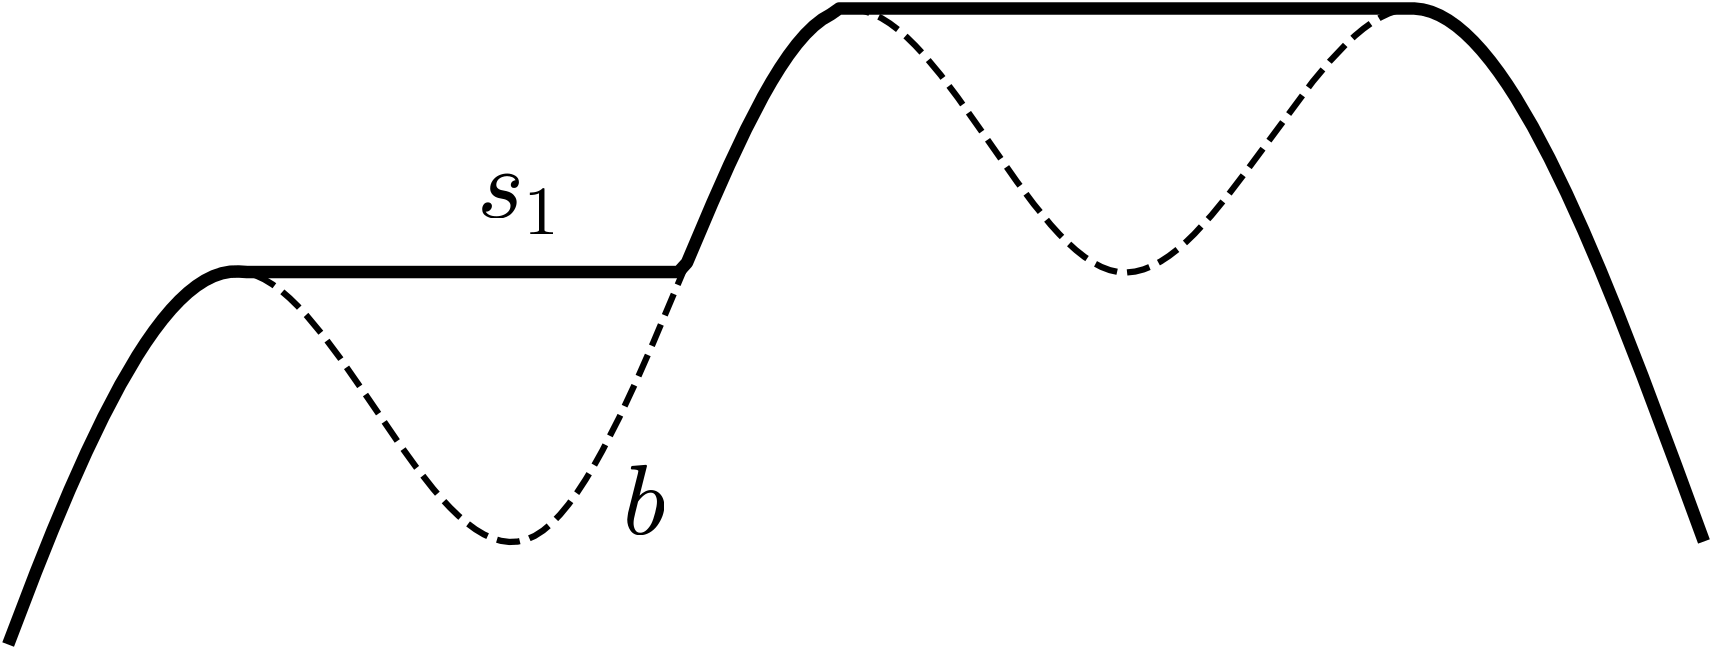
\includegraphics[width=0.4\textwidth]{genfigs/filled.pdf} \qquad 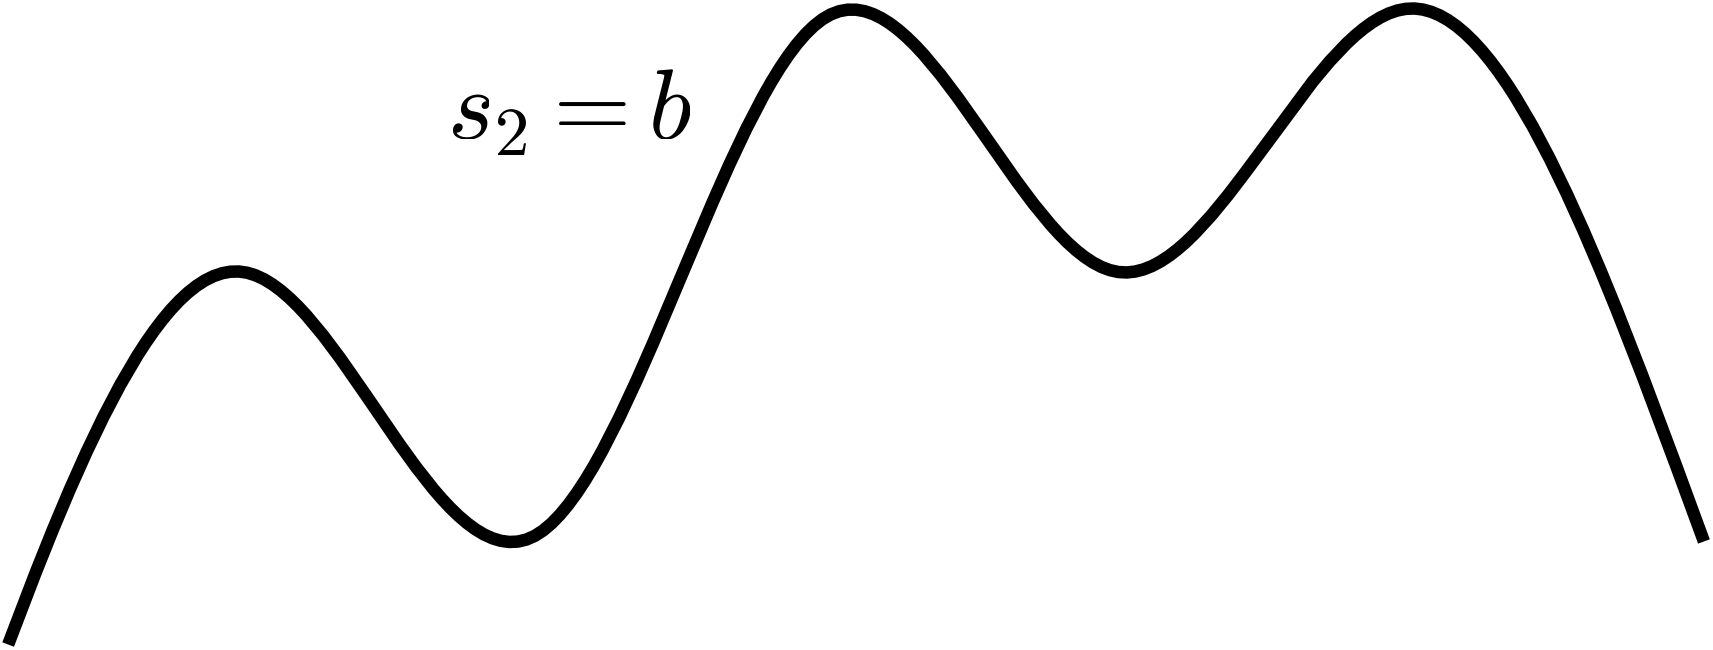
\includegraphics[width=0.4\textwidth]{genfigs/icefree.pdf}}
\end{center}
\caption{For a smooth bedrock elevation $b$ with local minima, a surface elevation state $s_1$ that fills-in the minima with flat ice (left) gives zero surface velocity in a Stokes model: $\bu|_{s_1}=\bzero$.   The ice-free state $s_2=b$ (right) likewise has $\bu|_{s_2}=\bzero$.  This shows that the surface motion map $\Phi$ defined in \eqref{eq:definePhi} is not coercive.}
\label{fig:noncoercive}
\end{figure}

Two consequences of this construction are now stated as propositions.

\begin{proposition} \label{prop:noncoercive}
The surface motion map $\Phi$ defined in \eqref{eq:definePhi} is not $q$-coercive (Definition \ref{def:monotonecoercive}), for any $q$, nor is it strictly-monotone.
\end{proposition}

\begin{proof}
Note $(\Phi(s_1) - \Phi(s_2))[s_1-s_2]=0$ while $\alpha \|s_1-s_2\|_\cX > 0$.
\end{proof}

\begin{proposition} \label{prop:notunique}
When the SMB is identically zero, $a=0$, there are smooth bedrock elevations for which the steady-state version of a glacier geometry model will have more than one solution.
\end{proposition}

\begin{proof}
The NCP form of the steady-state and $a=0$ model in question is
	$$s - b \ge 0, \quad - \bu|_s \cdot \bn_s \ge 0, \quad (s - b) \left(- \bu|_s \cdot \bn_s\right) = 0,$$
with corresponding weak form over $s\in\cK\subset\cX$.  If $b$ is a smooth function with local minima then the above construction of $s_1$ and $s_2$ gives distinct solutions.
\end{proof}
Proposition \ref{prop:notunique} answers negatively the uniqueness question which has been open since the existence theorem for the general-bed, steady shallow ice approximation \cite{JouvetBueler2012}.  It uses a surprisingly-simple construction, but one which seems not to appear in the literature.  Non-uniqueness here happens for a SMB function which is elevation \emph{in}dependent, namely $a=0$.  This result is different from the better-known non-uniqueness \cite{Bodvardsson1955} and non-existence \cite{Jouvetetal2011} results for certain elevation-dependent SMB models.


\section{Experiments on coercivity of the surface motion map} \label{app:numerical}

Conjecture \ref{conj:c} is needed in the proposed well-posedness framework for the continuum implicit time-step problem for glaciers (Sections \ref{sec:stokes}--\ref{sec:conjectural}).  It is also critical to the application of \emph{a priori} Theorem \ref{thm:abstractestimate}, which hypothesizes coercivity, as our main goal is to bound surface elevation errors in FE simulations (Section \ref{sec:application}).

The reasonableness of this Conjecture can be tested by sampling from simulations.  The numerical experiments here, using Python and the Firedrake FE library \cite{Hametal2023},\footnote{Source code is at the public repository \href{https://github.com/bueler/glacier-fe-estimate}{\texttt{github.com/bueler/glacier-fe-estimate}}, in the \texttt{py/} directory.  The codes call the library at \href{https://github.com/bueler/stokes-extrude}{\texttt{github.com/bueler/stokes-extrude}}.} were not intended to demonstrate time-stepping.  They simply generated admissible surface elevation pairs $\sigma,s\in\cK \subset \cX = W^{1,4}(\Omega)$, to use as samples in a coercivity test.  For each pair we evaluated the coercivity ratios
\begin{equation}
\rho^\eps(\sigma,s) = \frac{\left(\Phi^\eps(\sigma) - \Phi^\eps(s)\right)[\sigma-s]}{\|\sigma-s\|_{\cX}^4}. \label{eq:Phiratio}
\end{equation}
We evaluated \eqref{eq:Phiratio} as written, based on formula \eqref{eq:defineregularizedPhi} and $\eps=0.1$, and as the original surface motion map \eqref{eq:definePhi}, i.e.~for $\eps=0$.  Note that while Appendix \ref{app:noncoercive} shows there exist pairs that give $\rho^0(\sigma,s)>0$, they generate $\rho^\eps(\sigma,s)>0$ when $\eps>0$.

If the set of all possible ratios $\{\rho^\eps(\sigma,s)\}$ were bounded below by a positive constant $\alpha>0$, then this fact would confirm bound \eqref{eq:conj:c} and Conjecture \ref{conj:c}.  However, a numerical experiment obviously allows only finite sampling of the ratios, and particulars of data and discretization must be selected.  Here the domain is the 1D interval $\Omega=(-L,L)$ with $L=100$ km, meshed into equal intervals.  The FE space $\cX_h\subset \cX$ is the set of continuous $P_1$ (piecewise-linear) functions.  For $b,s\in\cX_h$ the Stokes domain $\Lambda(s)$ is thus polygonal; see \eqref{eq:domainfroms}.  Regarding the data, two bed profiles (Figure \ref{fig:cases}) are considered, \emph{flat} ($b_1(x)=0$) and \emph{rough} ($b_2(x)$), and three constant SMB values $a_j\in\{-2.5,0.0,1.0\}\times 10^{-7}$\, $\text{m}\,\text{s}^{-1}$.  The $b_2$ bed is a linear combination of several sinusoids down to 4 km wavelength.

\begin{figure}[ht]
\centering
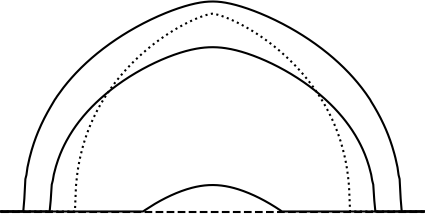
\includegraphics[width=0.35\textwidth]{figs/snapsflat.png} \quad 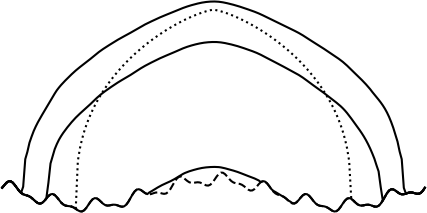
\includegraphics[width=0.37\textwidth]{figs/snapsrough.png}
\caption{Two bed profiles (dashed; flat on left and rough on right) define constraint sets ${\cK_h}_i\subset\cX_h$, $i=1,2$, in the numerical experiment.  For each ${\cK_h}_i$, runs using different constant values of the SMB (see text) generated a large number of admissible surface elevations, with a few shown here, representing large and small glaciers covering different portions of the domain.}
\label{fig:cases}
\end{figure}

Using definition \eqref{eq:be:admissible}, each bed elevation $b_i$, $i=1,2$, generated a constraint set ${\cK_h}_i \subset \cX_h$.  A time-dependent, Stokes-dynamics simulation of $T=200$ years was done for each combination of set ${\cK_h}_i$ and value $a_j$.  One thousand sample pairs were taken from the three runs with a given ${\cK_h}_i$, at random times in $[0,T]$, with samples coming equally from different $a_j$ runs.  Because the $a_j$ values caused advance or retreat of the ice margins, and indeed for $a_1<0$ the glacier actually disappears, the computed ratios came from both similar surface elevation pairs and very different pairs.  The initial surface for these runs is a Halfar profile \cite{Halfar1981} (Figure \ref{fig:cases}, dotted).  For the $b_1=a_2=0$ case the exact time-dependent surface elevation solution \emph{under shallow dynamics} is therefore known.  Though Stokes dynamics was used in the numerical experiment, the final surface agrees closely with this shallow exact solution; compare \cite{LofgrenAhlkronaHelanow2022}.

In these simulations each time-step was semi-implicit, approximating VI \eqref{eq:be:vi} by using $\bu|_{s^{n-1}}\cdot\bn_{s^n}$ as mentioned in the Introduction.  The stabilization technique from \cite{LofgrenAhlkronaHelanow2022} was also applied.  The VIs were then solved using a reduced-space Newton method with line search \cite{BensonMunson2006}.  The Stokes problems \eqref{eq:glenstokes:weak}, with viscosity regularization $\mu_0=10^{-19}\, \text{s}^{-2}$ in \eqref{eq:glen}, were solved on the domains $\Lambda(s^{n})$ using a vertically-extruded mesh of quadrilaterals (Figure \ref{fig:fe:operatorvisualization}), a $Q_2\times Q_1$ (Taylor-Hood stable pair \cite{Elmanetal2014}) mixed FE method, and a Newton solver, with direct solution of the linear step equations.  The resulting time-dependent numerical method is only conditionally-stable \cite{LofgrenAhlkronaHelanow2022}, but it is adequate for our purpose of generating sample surface elevations.

The basic result of these experiments is in Figure \ref{fig:regratios}, which shows sample ratios $\rho^{0.1}(\sigma,s)$, i.e.~\eqref{eq:Phiratio} for $\eps=0.1$, as histograms on a logarithmic axis.  These are from the highest spatial resolution, $\Delta x=500$ m and 40 elements in each (extruded) column.  More than $99\%$ of the ratios are positive for the flat bed (${\cK_h}_1$), and all are positive for the more-generic rough bed (${\cK_h}_2$).  For the latter a coercivity constant $\alpha=10^{-22}$ is credible.  Note that dimensional values around $10^{-20}$ are expected because $\|s\|_{\cX}\sim 10^{5}$ is typical for these surfaces, in the Sobolev space $\cX = W^{1,4}(\Omega)$ using consistent norm scaling \eqref{eq:norm:Omega}, while the residuals in the numerator of \eqref{eq:Phiratio} have typical magnitudes between $10^{-5}$ and one.

\begin{figure}[ht]
\centering
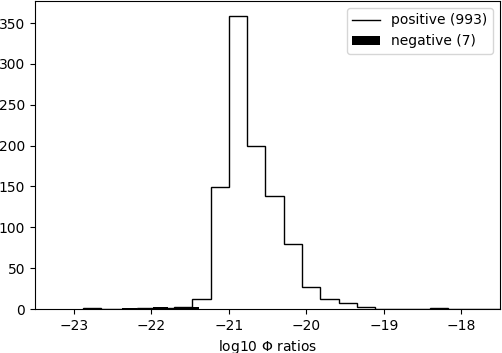
\includegraphics[width=0.40\textwidth]{figs/bflat500mREG.png} \, 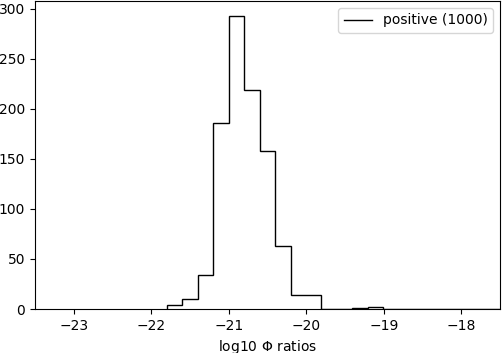
\includegraphics[width=0.40\textwidth]{figs/brough500mREG.png}
\caption{Histograms of ratios $\rho^{0.1}(\sigma,s)$ for 1000 sample pairs $\sigma,s$ from the flat-bed (left; ${\cK_h}_1$) and rough-bed (right; ${\cK_h}_2$) constraint sets.}
\label{fig:regratios}
\end{figure}

An underlying reason for evidence of coercivity in the regularized case is that \emph{the regularization does not need to do much work}.  Figure \ref{fig:noregratios} shows ratio histograms from the same sample pairs, but computed without regularization.  About $10\%$ are negative ($\rho^0(\sigma,s)<0$), which violates coercivity, but their absolute values are grouped about two orders of magnitude smaller than the positive ratios. Glacier evolution under Stokes dynamics seemingly wants to be coercive.  In fact, the continuum problem may be more coercive than a discretization.  Figure \ref{fig:resolutionratios} shows the results from running the same rough-bed experiment, at right in Figure \ref{fig:regratios}, but at lower $\Delta x=1000,2000$ m horizontal resolutions, with correspondingly lower vertical resolution as well.  These poorer discretizations produced many more negative ratios $\rho^\eps(\sigma,s)$; apparently spatial refinement improves coercivity.  Margin approximation improvements, for example via adaptive/local mesh refinement focussed near the free boundary \cite{FochesattoBueler2025}, should further improve the numerical evidence for coercivity.

\begin{figure}[ht]
\centering
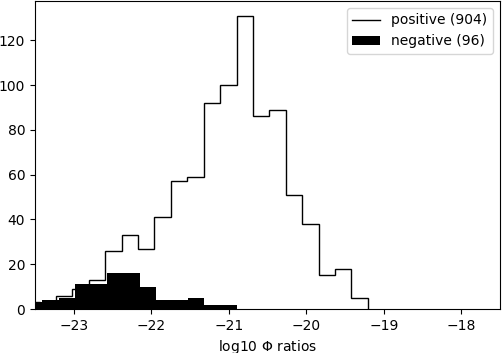
\includegraphics[width=0.40\textwidth]{figs/bflat500mNOREG.png} \, 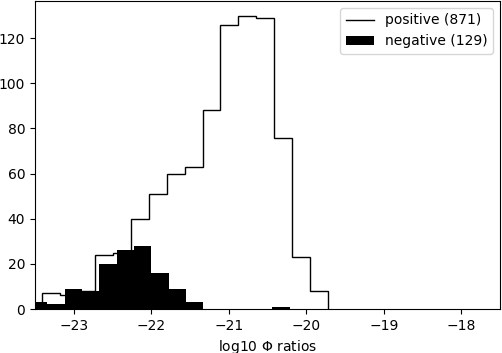
\includegraphics[width=0.40\textwidth]{figs/brough500mNOREG.png}
\caption{Histograms of ratios $|\rho^0(\sigma,s)|$ for the same sample pairs as in Figure \ref{fig:regratios}.}
\label{fig:noregratios}
\end{figure}

\begin{figure}[ht]
\mbox{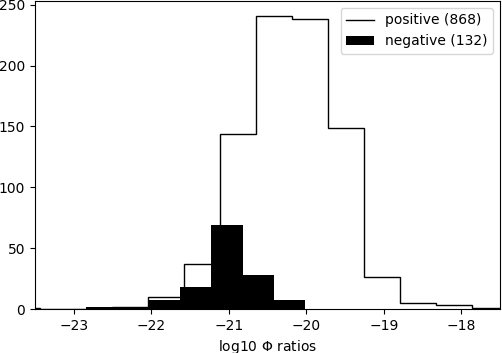
\includegraphics[width=0.31\textwidth]{figs/brough2000mREG.png} \, 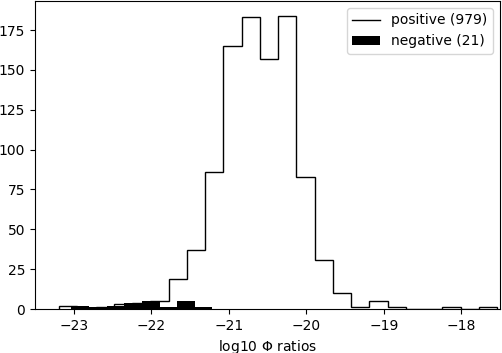
\includegraphics[width=0.31\textwidth]{figs/brough1000mREG.png} \, 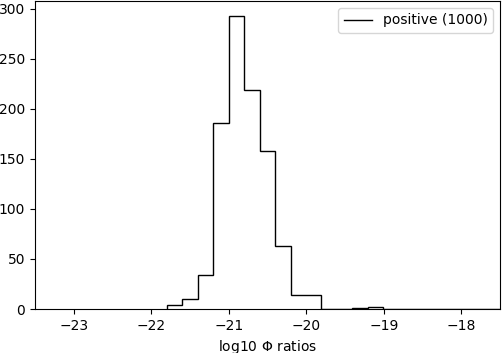
\includegraphics[width=0.31\textwidth]{figs/brough500mREG.png}}
\caption{The effect of resolution: Histograms of ratios $|\rho^{0.1}(\sigma,s)|$ for horizontal mesh resolutions $\Delta x=2000$ m (left), $1000$ m (middle), and $500$ m (right; same as Figure \ref{fig:regratios} right).}
\label{fig:resolutionratios}
\end{figure}

% flat: 2.576e-07
% rough: 2.230e-07
Regarding Conjecture \ref{conj:b}, Lipschitz continuity for the surface velocity trace, the maximum of the relevant ratio $\big\|\bu|_\sigma - \bu|_s\big\|_{L^{4/3}}/\|\sigma-s\|_{W^{1,4}}$ was found to be $2.6\times 10^{-7}$ for the same sample pairs as in Figure \ref{fig:regratios}.  Of course, numerical experiments cannot prove this Conjecture either.

In summary we have substantial, but necessarily very incomplete, evidence for Conjecture \ref{conj:c}.  Recall that this Conjecture is an important aspect of well-posedness of the (spatially-continuous) implicit time-step VI problem \eqref{eq:be:vi}, and it is critical to the glaciers application of the \emph{a priori} error bound, that is, the result in Theorem \ref{thm:glacierapp}.

\end{document}
